
% Autor y título

\documentclass[12pt]{article}
\usepackage[utf8]{inputenc}
\usepackage[spanish,es-tabla,es-nodecimaldot]{babel}

% Paquetess

\usepackage{amsmath}
\usepackage{amsthm}
\usepackage{amsfonts}
\usepackage{amssymb}
\usepackage{makeidx}
\usepackage{graphicx}
\usepackage{lmodern}
\usepackage[dvipsnames]{xcolor} 
\usepackage{fancyhdr}
\usepackage{geometry}
\usepackage{lastpage}		
\usepackage{array}			 % Para fjar tamaño de columnas
\usepackage{tikz}
\usepackage{subcaption}
\usepackage{caption}
\usepackage{pgfplots} % Para controlar la perspectiva
\RequirePackage{siunitx}
\usepackage{extramarks} % Para poder usar firstleftmarks
\usepackage[version=4]{mhchem} % Para poder usar formulas de reacciones nucleares
\usepackage{chemfig}
\usepackage{xcolor}
\RequirePackage[most]{tcolorbox}
\usepackage{enumitem}
\usepackage{physics}
%\usepackage{background}
\usepackage{eso-pic} % Para insertar imágenes de fondo específicas
\usepackage[absolute,overlay]{textpos} % Paquete para colocar elementos en posiciones absolutas
\usepackage{wrapfig}
\usepackage{booktabs}
\usepackage{float} % en el preámbulo
\usepackage{lipsum}
\usepackage{adjustbox} % en el preámbulo
\usepackage{etoolbox} % asegúrate de incluir esto

\usepackage{listings}
\usepackage{courier}
\usepackage{color}
\usepackage[normalem]{ulem} % para subrayado
\usepackage{soul}
\sethlcolor{red!30}


\AtBeginEnvironment{table}{\scriptsize} % cambia \small por \footnotesize, \scriptsize, etc.


\setlength{\parindent}{0pt} % Elimina la sangría
\newtcolorbox{mybox}{colback=black!5!white,
	colframe=black!75!black}

\newtcolorbox{Anotacion}{colback=red!5!white,
	colframe=red!75!red}


%##############################################################################
%######### Ponemos el decimal con . ###########################################
%##############################################################################

\sisetup{output-decimal-marker={.},
	% exponentes ------------------------
	exponent-mode=threshold,
	exponent-thresholds=-3:4, % non usar exponentes 10^{-2,-1, 0, 1,2,3}
	% redondear -------------------------
	% round-mode=figures, % cifras sig
	% round-mode=places, % cantos decimales
	round-mode=uncertainty, % cifras sig da incerteza (necesario usar erro)
	round-precision=2,
	%uncertainty-mode = separate,
	print-unity-mantissa=false,
	% unidades --------------------------
	inter-unit-product = \ensuremath{{}\cdot{}}, % separacion entre unidades
	% per-mode=power-positive-first, % so furrula con metodo interpretado puro
	inline-per-mode=single-symbol,
	display-per-mode=fraction,
}

%##############################################################################
%######### Para codigo python #################################################
%##############################################################################

\definecolor{codegreen}{rgb}{0,0.6,0}
\definecolor{codegray}{rgb}{0.5,0.5,0.5}
\definecolor{codepurple}{rgb}{0.58,0,0.82}

\usepackage{listings}


\definecolor{mygreen}{rgb}{0,0.6,0}
\definecolor{mygray}{rgb}{0.5,0.5,0.5}
\definecolor{mymauve}{rgb}{0.58,0,0.82}
\lstset{ %
  backgroundcolor=\color{white},   % choose the background color; you must add \usepackage{color} or \usepackage{xcolor}
  basicstyle=\footnotesize\ttfamily,        % the size of the fonts that are used for the code
  breakatwhitespace=false,         % sets if automatic breaks should only happen at whitespace
  breaklines=true,                 % sets automatic line breaking
  captionpos=b,                    % sets the caption-position to bottom
  commentstyle=\color{mygreen},    % comment style
  deletekeywords={...},            % if you want to delete keywords from the given language
  escapeinside={\%*}{*)},          % if you want to add LaTeX within your code
  extendedchars=true,              % lets you use non-ASCII characters; for 8-bits encodings only, does not work with UTF-8
  frame=single,                    % adds a frame around the code
  keepspaces=true,                 % keeps spaces in text, useful for keeping indentation of code (possibly needs columns=flexible)
  keywordstyle=\color{blue},       % keyword style
  language=Python,                 % the language of the code
  otherkeywords={*,...},            % if you want to add more keywords to the set
  numbers=left,                    % where to put the line-numbers; possible values are (none, left, right)
  numbersep=5pt,                   % how far the line-numbers are from the code
  numberstyle=\tiny\color{mygray}, % the style that is used for the line-numbers
  rulecolor=\color{black},         % if not set, the frame-color may be changed on line-breaks within not-black text (e.g. comments (green here))
  showspaces=false,                % show spaces everywhere adding particular underscores; it overrides 'showstringspaces'
  showstringspaces=false,          % underline spaces within strings only
  showtabs=false,                  % show tabs within strings adding particular underscores
  stepnumber=2,                    % the step between two line-numbers. If it's 1, each line will be numbered
  stringstyle=\color{mymauve},     % string literal style
  tabsize=2,                       % sets default tabsize to 2 spaces
  title=\lstname                   % show the filename of files included with \lstinputlisting; also try caption instead of title
}

%%%%%%%%%%%%%%%%%%%%%%%%%%%%%%%%%%%%%%%%%%
%%%%%%%%%%%%%%%%%% BIBLIOGRAFIA %%%%%%%%%%
%%%%%%%%%%%%%%%%%%%%%%%%%%%%%%%%%%%%%%%%%%


\usepackage{biblatex} %Imports biblatex package
\addbibresource{sample.bib} %Import the bibliography file

%##############################################################################
%######### Tipo de fuente #################################################
%##############################################################################

%\usepackage{newtxtext,newtxmath} % Cambia la fuente (pero mola)
\RequirePackage{libertinus} % Cambia la fuente -> Papers
\RequirePackage{mathptmx}   % Loads the Times-Roman Math Fonts


%\usepackage{kpfonts}
%\usepackage{helvet} 
%\renewcommand{\familydefault}{\sfdefault}.

%\usepackage{fontspec} % Paquete necesario para seleccionar fuentes
%\setmainfont{Verdana} % Cambia la fuente principal a Verdana


%##############################################################################
%######### Geometría #################################################
%##############################################################################

%\geometry{a4paper, total={169mm,245mm}, left=20mm, top=30mm}
\geometry{a4paper,left=2cm,right=2cm,top=2.5cm,bottom=2.5cm}



%##############################################################################
%######### Formatos capítulo #################################################
%##############################################################################

%\usepackage[lmodern]{quotchap}
%\usepackage[options]{fncychap}
% Configuración de la imagen de fondo solo para la portada


%##############################################################################
%######### Hiperreferenias #################################################
%##############################################################################

\usepackage[colorlinks=true, linkcolor=Blue, citecolor=ForestGreen, urlcolor=BrickRed]{hyperref} % Crea las
\usepackage[nameinlink]{cleveref}
\crefname{figure}{fig.}{Figs.}
\crefname{table}{tab.}{Tabs.}

%##############################################################################
%######### Formato de pagina #################################################
%##############################################################################

\pagestyle{fancy}
\fancyhf{} % Limpia encabezados y pies
\fancyhead[L]{\small \textbf{Trabajo de Fin de Grado}}    % Encabezado izquierdo
\fancyhead[R]{\small \textbf{Daniel Vázquez Lago}}     % Encabezado derecho
\fancyfoot[C]{\thepage}      % Pie de página centrado con el número de página
\renewcommand{\headrulewidth}{0.4pt}  % Grosor de la línea del encabezado
\renewcommand{\footrulewidth}{0pt}    % Sin línea en el pie
\usepackage{etoolbox} % asegúrate de incluir esto

\AtBeginEnvironment{table}{\small} % cambia \small por \footnotesize, \scriptsize, etc.



%##############################################################################
%#########  Modificar caption #################################################
%##############################################################################

\usepackage[font=small, justification=justified]{caption}  % Configura las captions



%##############################################################################
%######### Comandos propios #################################################
%##############################################################################


\newcommand{\parentesis}[1]{\left( #1  \right)}
\newcommand{\parciales}[2]{\frac{\partial #1}{\partial #2}}
\newcommand{\pparciales}[2]{\parentesis{\parciales{#1}{#2}}}
\newcommand{\ccorchetes}[1]{\left[ #1  \right]}
\newcommand{\D}{\mathrm{d}}
\newcommand{\derivadas}[2]{\frac{\D #1}{\D #2}}

\newcommand{\tquad}{\quad \quad \quad}
%\newcommand{\vnabla}{\vec{\nabla}}

\newcommand{\Ocal}{\mathcal{O}}
\newcommand{\Jcal}{\mathcal{J}}
\newcommand{\Mcal}{\mathcal{M}}
\newcommand{\Fcal}{\mathcal{F}}
\newcommand{\Hcal}{\mathcal{H}}
\newcommand{\Ecal}{\mathcal{E}}
\newcommand{\Ncal}{\mathcal{N}}

\newcommand{\cmm}{\text{cm}^{-1}}
\newcommand{\fcc}{\textit{fcc}}
\newcommand{\bcc}{\textit{bcc}}
\renewcommand{\sc}{\textit{sc}}
\newcommand{\hcp}{\textit{hcp}}


\newcommand{\PZB}{\text{{\tiny PZB}}}
\newcommand{\gap}{\text{{\tiny gap}}}
\newcommand{\SZB}{\text{{\tiny SZB}}}
\newcommand{\inicial}{\text{{\tiny inicial}}}
\newcommand{\final}{\text{{\tiny final}}}
\newcommand{\atomico}{\text{{\tiny atómico}}}

\newcommand{\arctanh}{\text{{arctanh}}}



\newcommand{\Namas}{\text{Na}^+}
\newcommand{\Clmenos}{\text{Cl}^-}

\newcommand{\cm}{\text{cm}}
\newcommand{\eV}{\text{eV}}

\newcommand{\arr}{\text{arr}}
\newcommand{\diff}{\text{diff}}

\newcommand{\er}{$^{\text{er}}$}
\newcommand{\cte}{\text{cte}}
\newcommand{\expo}{\text{exp}}
\newcommand{\simu}{\text{sim}}


% Comandos vectoriales

\newcommand{\an}{\mathbf{a}}
\newcommand{\bn}{\mathbf{b}}
\newcommand{\dn}{\mathbf{d}}
\newcommand{\fn}{\mathbf{f}}
\newcommand{\jn}{\mathbf{j}}
\newcommand{\kn}{\mathbf{k}}
\newcommand{\pn}{\mathbf{p}}
\newcommand{\qn}{\mathbf{q}}
\newcommand{\rn}{\mathbf{r}}
\newcommand{\sn}{\mathbf{s}}
\newcommand{\un}{\mathbf{u}}
\newcommand{\vn}{\mathbf{v}}
\newcommand{\xn}{\mathbf{x}}
\newcommand{\wn}{\mathbf{w}}
\newcommand{\yn}{\mathbf{y}}
\newcommand{\qndot}{\dot{\qn}}

\newcommand{\alphan}{\boldsymbol{\alpha}}
\newcommand{\sigman}{\boldsymbol{\sigma}}
\newcommand{\pin}{\boldsymbol{\pi}}
\newcommand{\rhon}{\boldsymbol{\rho}}
\newcommand{\epsilonn}{\boldsymbol{\epsilon}}
\newcommand{\omegan}{\boldsymbol{\omega}}
\newcommand{\mun}{\boldsymbol{\mu}}



\newcommand{\An}{\mathbf{A}}
\newcommand{\Bn}{\mathbf{B}}
\newcommand{\En}{\mathbf{E}}
\newcommand{\Fn}{\mathbf{F}}
\newcommand{\Jn}{\mathbf{J}}
\newcommand{\Hn}{\mathbf{H}}
\newcommand{\Gn}{\mathbf{G}}
\newcommand{\Kn}{\mathbf{K}}
\newcommand{\Ln}{\mathbf{L}}
\newcommand{\Mn}{\mathbf{M}}
\newcommand{\Pn}{\mathbf{P}}
%\newcommand{\Rn}{\mathbf{R}}
\newcommand{\Sn}{\mathbf{S}}
\newcommand{\Tn}{\mathbf{T}}
\newcommand{\In}{\mathbf{1}}
\newcommand{\Encal}{\boldsymbol{\mathcal{E}}}

\newcommand{\hnn}{\hat{\mathbf{n}}}
\newcommand{\hnr}{\hat{\mathbf{r}}}
\newcommand{\hnz}{\hat{\mathbf{z}}}
\newcommand{\hnv}{\hat{\mathbf{v}}}
\newcommand{\hnx}{\hat{\mathbf{x}}}
\newcommand{\hny}{\hat{\mathbf{y}}}
\newcommand{\hnu}{\hat{\mathbf{u}}}
\newcommand{\hnR}{\hat{\mathbf{R}}}
\newcommand{\hnp}{\hat{\mathbf{p}}}
\newcommand{\hnk}{\hat{\mathbf{k}}}
\newcommand{\hni}{\hat{\mathbf{i}}}
\newcommand{\hnj}{\hat{\mathbf{j}}}
\renewcommand{\hnk}{\hat{\mathbf{k}}}

%%%%%%%%%%%%%%%%%%%%%%%%%%%%%%%%%%%%%%%%%%%%%%%%%%%%%%%%%%%%%%
%%%%%%%%%%%%%%%%%%%%%%% COMIENZA %%%%%%%%%%%%%%%%%%%%%%%%%%%%%
%%%%%%%%%%%%%%%%%%%%%%%%%%%%%%%%%%%%%%%%%%%%%%%%%%%%%%%%%%%%%%
 
\title{\textbf{\Huge Trabajo de Fin de Grado}}
\author{\Large Daniel Vázquez Lago}
\date{\today}
			

\begin{document}

\maketitle
\newpage
\tableofcontents
\newpage

\setlength{\parskip}{2.2mm} % Cambia el espacio entre párrafos



\section{Objetivos y motivación}

Cita de prueba: \cite{key}. \\

El objetivo principal de esta práctica es estudiar mediante simulaciones el comportamiento de la siguiente reacción nuclear:

\begin{equation}
	^{11}\mathrm{Li}+^2\mathrm{H} \rightarrow ^3\mathrm{H}+^{10}\mathrm{Li} \Longleftrightarrow 1 + 2 \rightarrow 3 + 4
\end{equation}

Esta reacción es de alto interés en la física nuclear, ya que permite estudiar
\section{Motivación experimental}



\subsection{Modelo de capas}

La hipótesis principal del modelo de capas es suponer que los nucleones se mueven en el núcleo casi independientemente los unos de los otros a pesar de la interacción fuerte. Este movimiento libre significa, en última instancia, que el recorrido libre medio de un nucleón en materia nuclear es grande comparado con las dimensiones del núcleo. En el modelo de capas la interacción nucleón con sus compañeros se reduce a la interacción con un \textbf{campo autoconsciente} (\textit{self-consistent field}) creado por ellos. Generalmente se supone que este campo autoconsciente es estático y esféricamente simétrico.

Debido al corto alcance de las fuerzas nucleares, el potencial del campo autoconsciente tiene dependencia radial muy similiar a la densidad nuclear, es decir, es casi constante dentro del núcleo y se anula fuera. Por lo tanto, en primera aproximación podríamos considerar que el potencial nuclear constante en el interior del núcleo, tal como se hace en el modelo de gas de Fermi ideal\footnote{El modelo de capas incorpora la hipótesis del modelo de gas de Fermi.}, con lo cual las funciones de onda de los nucleones serían ondas planas.

No obstante, cuando introducimos un campo autoconsistente que depende de la distancia al centro del núcleo, las funciones de onda de los nucleones se modifican, a través de la ecuación de Schrödinger, dejando de ser ondas planas. Una vez definido el potencial con el que queramos modelar la interacción nuclear, las soluciones nos llevarán a estados energéticos discretos similares, que como en el caso del átomo de hidrógeno, irá llenando los niveles energéticos de acuerdo con el principio de Pauli. El potencial uisado es la suma del potencial de Coulomb, un potencial que contenga la interacción nuclear (el más realista es un potencial de Wood-Saxon) y el término de interacción espín-órbita. A través de estos niveles podemos predecir el valor tanto del momento angular total y los posibles estados excitados del núcleo. Existen varias secuencias de llenado de nucleones en la literatura, dependiendo de los parámetros exactos que se usen en la parametrización del campo nuclear autoconsciente. Por ejemplo, usando un potencial nuclear parametrizado como un armónico con término quadrupolar de tal modo que podamos incluir un parámetro que incluya la deformación del núcleo tendríamos una correción del modelo de capas, en el llamado \textit{modelo de Nilsson} \cite{Nilsson:212345}, o por ejemplo el modelo Seniority o BCS \cite{Broglia} que incluye términos de apareamiento. 


En general este es capaz de predecir la mayoría de números mágicos \footnote{Que son ciertos valores de $N$ y $Z$ los núcleos muestran una estabilidad inusual, que se manifiesta, por ejemplo, en una energía de separación de dos nucleones (protones o neutrones) grande.}. Este tipo de modelos funciona muy bien para los núcleos estables, sin embargo no parece predecir correctamente los momentos angulares orbitales y de espín en núcleos exóticos debido a que es necsario incluir más términos en el potencial. Incluir más términos llevará a un reodenamiento de los niveles nucleares que puede cambiar drásticamente las energías de las excitaciones o momentos angulares de las mismas. Precisamente por eso importante estudiar núcleos exóticos, para comparar las predicciones de los modelos nucleares con datos experimentales y así evaluar la validez y las limitaciones del modelo de capas tradicional. Por ello, el estudio de estos sistemas no solo permite entender mejor la estructura nuclear, sino también refinar las herramientas teóricas utilizadas para describirla.

%Por ejemplo, usando un potencial nuclear parametrizado como un armónico con término quadrupolar de tal modo que podamos incluir un parámetro que incluya la deformación del núcleo tendríamos una correción del modelo de capas, en el llamado \textit{modelo de Nilsson} \cite{Nilsson:212345}, o por ejemplo el modelo Seniority o BCS \cite{Broglia} que incluye términos de apareamiento. 



\subsection{Núcleos ricos en neutrones}

Los núcleos ricos en neutrones es uno de los campos de la física nuclear moderna, no solo porque son fundamentales a la hora de entender los procesos r astrofísicos \cite{THIELEMANN2011346}, (proceso de captura rápida de neutrones), los cuales parecen responsables de la creación de la mayor parte de núcleos muy pesados $(60<A)$, que se dan en la expansión tras un colapso del núcleo de una supernova, o la descompresión de la materia neutrónica emitida por la fusion de una estrella binaria compacta de neutrones; sino porque revelan nuevas estructuras nucleares (halos nucleares, modificación del orden de las capas nucleares y números mágicos...). 

Estas nuevas estrucutras nucleares ponen a prueba modelos teóricos y arrojan información necesaria para adaptar modelos fenomenológicos que permitirán obtener resultados teóricos a otros núcleos ricos en neutrones imposibles de medir en experiemntos actualmente por la incapacidad actual de producirlos (debido a su baja estabilidad y su falta de estados ligados). 

La mayor parte de estrucutrasa exóticas la encontramos en la la drip-line, tanto de protones, como de neutrones, sobre la que conocemos únicamente 8 o 9 elementos sobre ella, particularmente en los átomos ligeros. En aquellos que se ha alcanzado esta drip-line los núcleos presentan formas exóticas, comportamientos anómalos que no son vistos en núcleos en la estabilidad. Entre estos comportamientos encontramos los núcleos halo. 

Existen muchas maneras de obtener información acerca la dripline. Por un lado encontramos decaimientos beta, que nos permiten conocer la masa, espín y momentos angulares. Por otro lado las interacciones y secciones eficaces elásticas nos hablan acerca el radio y distribuciones de densidades, las distribuciones a diferentes enerǵias y momentos angulares la presencia de núcleos halo. Las reacciones inelásticas de trasferencia o resonancias elásticas nos pueden arrojar iformación acerca de estados nucleares no ligados \cite{JONSON20041}


\subsection{Núcleo halo}


El halo de neutrones es, en esencia, una manifestación del efecto túnel cuántico, que surge cuando un estado nuclear ligado se encuentra muy próximo al continuo energético \cite{tanihata2023halo}, es decir, a un estado no ligado, y que se entiende como una estrucutra formada por varios cuerpos (uno pesado llamado \textit{core} y varios ligeros) de manera similar a la órbita de un electrón alrededor del núcleo. A los núcleos formados por dos nucleones y un core, tal que el estado con un núcleón y un core es no ligado \cite{tanihata2023lowEnergyHalo} lo llamamos \textbf{núcleo Borremeano}, y podemos encontrar entre ellos $^6$He, $^{11}$Li, $^{14}$Be y $^{17}$B. 



Para que se de una estructura de halo se necesita una combinación de energía de ligadura de neutrones muy pequeña ($<1$ MeV) y una fuerza de corto alcanzce (como es la fuerza nuclear) \cite{tanihata2023halo}, que por ejemplo ene le caso del $^{11}$Li es de $S_{2n}=369.15(65)$ keV \cite{PhysRevLett.101.202501}. El requerimiento de que la energía de ligadura sea pequeña hace que la mayor parte de los halos solo puedan tener uno o dos neutrones en el halo. Dicha combinación de factores permite al neutrón a través del efecto túnel moverse alrededor del core nucleo, lo que conlleva a su vez que el núcleo tenga un tamaño más grande de lo normal: la función de ondas de los neutrones hace probable que este a distancias mucho más lejanas. 

Precisamente esto fue demostrado en 1985 por Tanihata et Al. para el $^{11}$Li, que por aquel entonces era un candidato a ser un núcleo halo. En este experimento hallaron que su radio era un 30\% mayor que el núcleo $^{9}$Li. Teóricamente este estado halo considearba que el core interaccionaba levemente con el núcleo, y que por tanto la distribución de carga debía ser similar entre el litio 9 y el litio 11. Esto fue probado por el ISOLDE, CERN, estudiando el momento cuadrupolar eléctrico \cite{ARNOLD199216} y momento tipolar magnético \cite{Arnold:180144} a través de decaimientos beta. Se había predicho además que la presencia de halos estarían asociadas a grandes secciones eficaces, lo cual también fue demostrado experimentalmente. 


\subsection{Litio 10 y Litio 11}

Como ya hemos dicho, el litio 11 es un núcleo borromeano, para lo cual es condición indispensable que el núcleo litio 10 sea un núcleo no ligado, es decir, que la suma de la masa de los protones y neutrones que la componen sea menor que la masa del propio litio 10. Que sea un estado no ligado implica que solo pueden vivir a través de 

¿Por qué es interesante conocer el estado no ligado litio 10? Por que las función de ondas del $^{11}$Li puede expresarse en realidad como una superposición de diferentes resonancias del $^{10}$Li y un neutrón que ocupa lo que denominamos ``estado orbital relevante'' o último estado orbital (el que define alguna de las características de interés del sistema) \cite{SANETULLAEV2016481}. Además de conocer el estado del litio 10, lo cual puede hacerse a través de varias reacciones, para conocer el litio 11 necesitaremos entender cuales son las relaciones del litio 10 y el neutrón extra.

En principio el litio 10 según el modelo de capas típico debería tener una componente principal de $1p_{1/2}$ tal y como mostramos en \cref{Fig:2-Li10_1}. sin embargo es sabido que debido a la gran cantidad de neutrones que hay en el sistema el modelo de capas habitual no funciona. El reordenamieno producido por el uso de términos adicionales, como puede ser el \textit{modelo de capas de Gamow} llevan a que el estado $2s_{1/2}$ se introduzca entre el $1p_{3/2}$  y el $1p_{1/2}$. 

\begin{minipage}{0.48\linewidth}
    \centering
    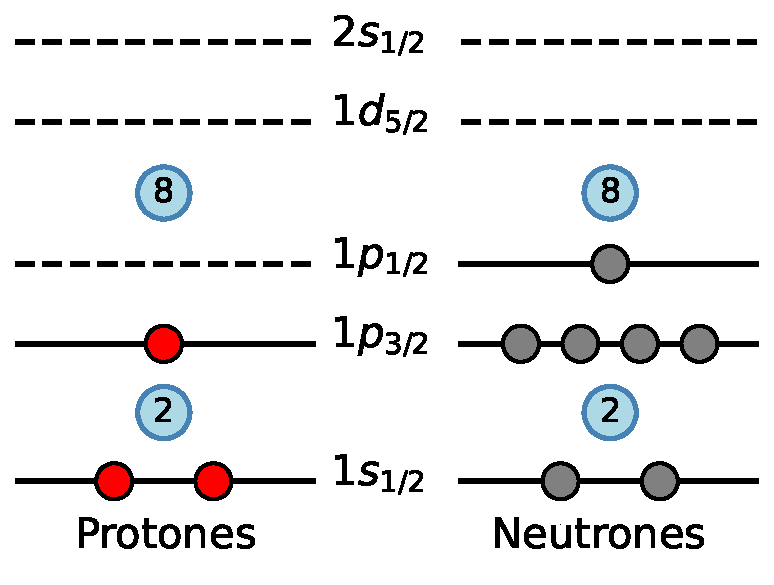
\includegraphics[width=1.0\linewidth]{Imagenes/Capas_10Li.pdf}
    \captionof{figure}{Capas del $^{10}$Li según el modelo de capas tradicional.}
    \label{Fig:2-Li10_1}
\end{minipage}
\hfill
\begin{minipage}{0.48\linewidth}
    \centering
    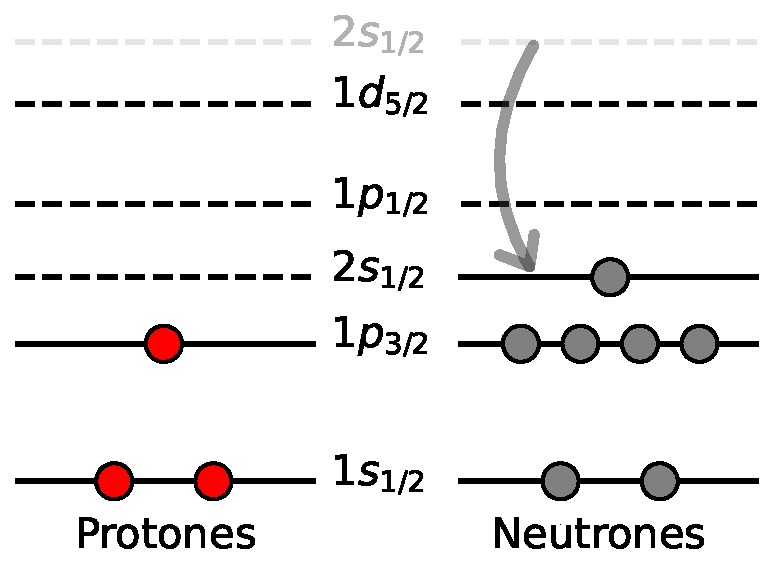
\includegraphics[width=1.0\linewidth]{Imagenes/Capas_10Li2.pdf}
    \captionof{figure}{Capas del $^{11}$Li según el modelo de capas modificado.}
    \label{Fig:2-Li10_2}
\end{minipage}

\vspace*{0.5cm}

Existen diferentes formas de explorar los estados resonantes, siempre a partir de reacciones de trasferencia, como $^{9}\text{Be}(^{9}\text{Be},^{8}\text{B})^{10}\text{Li}$. Diferentes reacciones se pusieron en marcha para poder hallar cual era el estado que dominaba, si el $1p_{1/2}$ o el $2s_{1/2}$, como pueden ser $^{9}\text{Li}(\text{d},\text{p})\text{Li}$ o $^{10}\text{Be}(^{12}\text{C},^{12}\text{N})^{10}\text{Li}$. La mayor parte de estas mostró que efectivamente el primer estado excitado es el $1p_{1/2}$ mientras qeu el estado fundamental era el $2s_{1/2}$. Pese a todo, la mayor parte de las reacciones no estudiaba que grado de influencia tenían estas resonancias en el $^{11}$Li \cite{SANETULLAEV2016481}.

Para esto, la mejor manera de hacerlo es a través de reacciones que quiten neutrones al $^{11}$Li, tal y como pueden ser  $^{11}$Li(p,d)$^{10}$Li o $^{11}$Li(d,t)$^{10}$Li. 




\subsection{Reacción de traferencia $^{11}$Li(d,t)$^{10}$Li}

La reacción en la que nos vamos centrar nosotros es: 

\begin{equation}
   {}^{11}\text{Li} + d \to t + {}^{10}\text{Li}
\end{equation}

Esta reacción es una de las más interesantes a la hora de obtener información acerca de núcleos halo con precisión. Esta es particularmente interesante dentro del estudio del litio 11 debido a su capacidad para proporcionar información directa sobre la estructura halo. A diferencia de muchas reacciones que sólo permiten estudiar el espectro excitado de \({}^{10}\text{Li}\), esta reacción accede directamente a las configuraciones de un solo neutrón en \({}^{11}\text{Li}\), facilitando la reconstrucción de sus componentes estructurales, tal y como hemos mencionado anteriormente.


¿Por qué es relevante estudiar \({}^{11}\text{Li}(d,t){}^{10}\text{Li}\)?
\begin{itemize}
    \item Permite investigar el papel de los estados resonantes de \(^{10}\text{Li}\) en la estructura del halo de \(^{11}\text{Li}\). Dado que $^{10}\text{Li}$ es inestable y no tiene un estado ligado, su estudio experimental es muy complicado, y esta reacción permite observar sus resonancias de forma más directa. \cite{SANETULLAEV2016481}.
    
    \item La transferencia de un neutrón desde \(^{11}\text{Li}\) al deuterón que forma el tritón permite poblar estados de \(^{10}\text{Li}\) con características específicas de momento angular y energía, mostrando la naturaleza de las configuraciones \(s_{1/2}\) y \(p_{1/2}\) en el estado fundamental de \({}^{11}\text{Li}\).  \cite{CASAL2017307}. 
    
    \item Es sensible a los factores espectroscópicos, es decir, permite medir la probabilidad de encontrar una cierta configuración de un neutrón y \({}^{10}\text{Li}\) en el estado fundamental de \({}^{11}\text{Li}\), lo cual no es accesible en muchas otras reacciones. \cite{SANETULLAEV2016481}. 
\end{itemize}

Ventajas frente a otras reacciones de transferencia
\begin{itemize}
    \item A diferencia de otras como \({}^{9}\text{Li}(d,p){}^{10}\text{Li}\), la reacción \({}^{11}\text{Li}(d,t){}^{10}\text{Li}\) accede directamente a la estructura del halo en \({}^{11}\text{Li}\), no sólo a la existencia de resonancias en \({}^{10}\text{Li}\). \cite{CASAL2017307}. 
    
    \item El modelo DWBA aplicado en este tipo de estudios, junto con funciones de solapamiento derivadas de un modelo tridimensional, permite una comparación más directa y realista con datos experimentales. \cite{CASAL2017307}.
\end{itemize}


En resumen, la reacción \({}^{11}\text{Li}(d,t){}^{10}\text{Li}\) no sólo aporta datos sobre los estados de \({}^{10}\text{Li}\), sino que se convierte en una herramienta crucial para entender cómo se configura el halo en \({}^{11}\text{Li}\), permitiendo extraer porcentajes de contribuciones tipo \(s_{1/2}\) y \(p_{1/2}\), y estudiar la ruptura del cierre de capa en \(N=8\). Por ello, tiene una relevancia singular dentro de la física nuclear de sistemas exóticos.


\section{Metodología}


\subsection{ACTAR TPC}

El detector ACTAR TPC (\textit{ACtive TARget and Time Projection Chamber}) es un detector diseñado para estudiar núcleos exóticos con tiempos de vida medios muy cortos, que con detectores tradicionales (en los que serían las partículas ligeras las que se acelerarían para bombardear al núcleo de interés) sería muy complicado.

Esto se debe a su funcionamiento en cinemática inversa, de tal modo que el núcleo pesado es el haz, lo que hace que la cinemática del centro de masas y del laboratorio sea muy diferente a la cinemática directa habitual, y por tanto su estudio de gran importancia. 

De esta forma, el gas que llena ACTAR TPC participa directamente en la reacción de interés y también como medio de detección (tal y como veremos mas adelante), confiriéndole su carácter de \textit{detector activo}. Es gaseoso por varios motivos: uno de ellos es poder usar la ionización de la partícula a través del gas para obtener trazas a partir del rastro de ionización que dejan todas las partículas cargadas. Bajo la presencia un campo eléctrico, los electrones de la ionización derivan hacia el ánodo, constituído por un detector segmentado en \textit{pads} donde se amplifica su carga. El tiempo de llegada de los electrones $\Delta t$ sirve de estimación de la posición $z$, conocida da velocidad de deriva del gas, un parámetro inherente a su presión y composición. Otro de los motivos es que conocemos con precisión el punto en el que sucedió la reacción (vértice), lo que no podríamos hacer en un experimento donde el \textit{target} fuera un sólido. Como las pérdidas de energía son bien conocidas \cite{ZIEGLER20101818}, conociendo el punto de inicio, el punto final de la partícula y la energía final, podemos obtener la energía de la partícula de salida en el vértice, lo cual nos permitirá calcular las variables cinemáticas (energías y ángulos) con gran precisión.

%En resumen, ACTAR TCP nos permite reconstruír tridimensionalmente el recorrido de la partícula dentro de la cámara de gas. Esta recostrucción 3D es la que permite obtener el vértice de la reacción y aplicar correciones por propagación.

Hablando de las características técnicas, ACTAR TPC tiene una dimensión de $606 \times 606 \times 335 $ mm$^3$, que sería toda la estructura azul violácea de la \cref{Fig:ACTAR}; con una caja en el interior de dimensiones $256 \times 256 \times 255 $ mm$^3$, llamada cámara de deriva, que es precisamente donde está el campo eléctrico que nos permite recolectar los electrones ionizados (en la parte superior) con detectores de $2 \times 2$ mm$^2$, y que en la \cref{Fig:ACTAR} sería la caja negra que está en el interior de la azul-violácea. Para nuestro experimento el interior lo llenaremos con una mezcla de dos gases: 90\% D$_2$ e 10\% CF$_4$ a una presión de 900 mbar (deuterio molecular y tetrafluorometano).

Debido a la cinemática de la reacción, existe una cierta probabilidad de que algunas partículas tengan suficiente energía como para atravesar el gas sin pararse, siendo imposible entonces reconstruir su energía en el vértice. Por eso se disponen a lo largo de los lados de ACTAR cuatro muros de silicios: dos en frente, en la dirección perpendicular al haz, y otros dos distribuidos a izquierda y derecha, como se ve en  \cref{Fig:Geo_Actar}. Cada muro está consituído por alrededor 10 unidades, de dimensiones $5 \times 5$ cm$^2$ $\times 1.5$ mm. Facilitan la medición de la energía residual de la partícula a la salida de la región activa, y su mecanismo de funcionamiento se describirá más adelante.

Se puede ver la disposición de los silicios usada en la \cref{Fig:Geo_Actar}. Estos silicios tuvieron que colocarse a una distancia prudencial de ACTAR $\sim 16.5$ cm, ya que aunque disminuya la eficiencia geométrica es posible que el campo eléctrico de los mismos distorsione el campo eléctrico de deriva. Consideraremos la notación l0 y r0 para los silicios de la izquierda y derecha respectivamente y f0  y f1 para la doble capa de silicios en la parte frontal.

\begin{minipage}{0.48\linewidth} \centering
	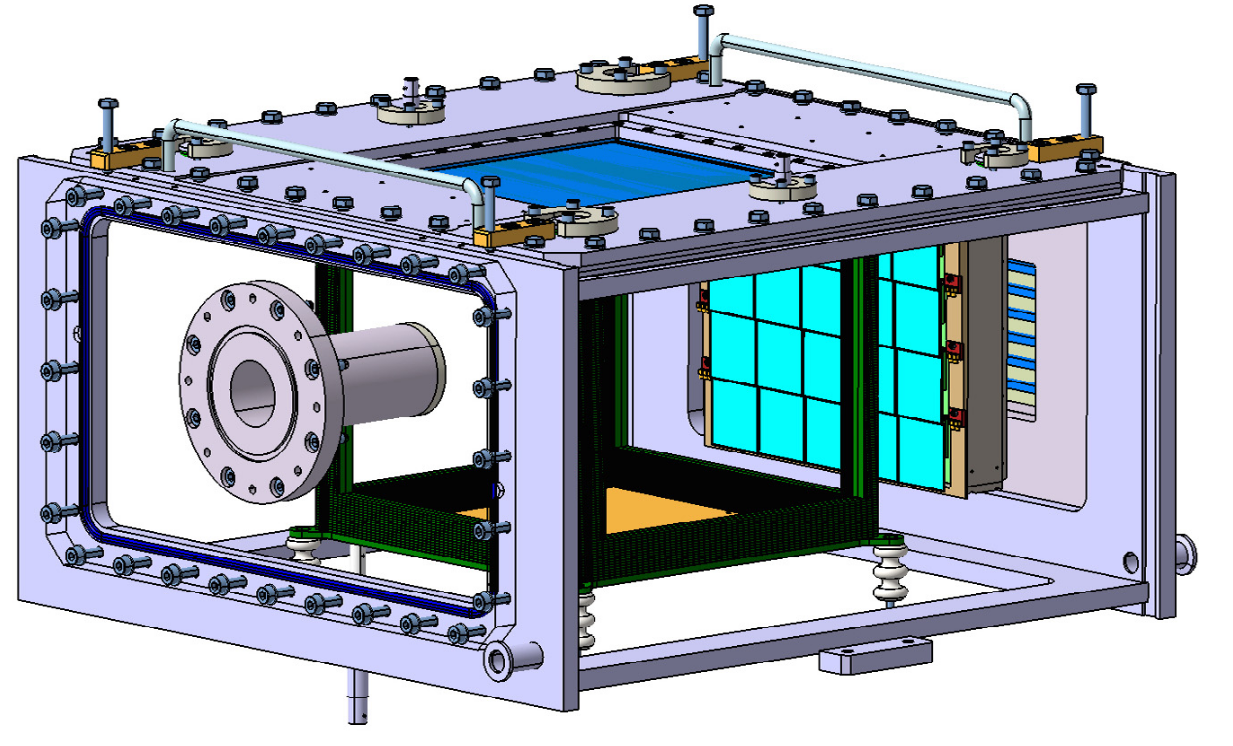
\includegraphics[width=1\linewidth]{Imagenes/ACTAR.png}
	\captionof{figure}{Dibujo en 3D asistido por ordenador (CAD) de ACTAR TPC. Imagen de \cite{MAUSS2019498}.}
	\label{Fig:ACTAR}
\end{minipage}
\hfill
\begin{minipage}{0.458\linewidth} \centering
	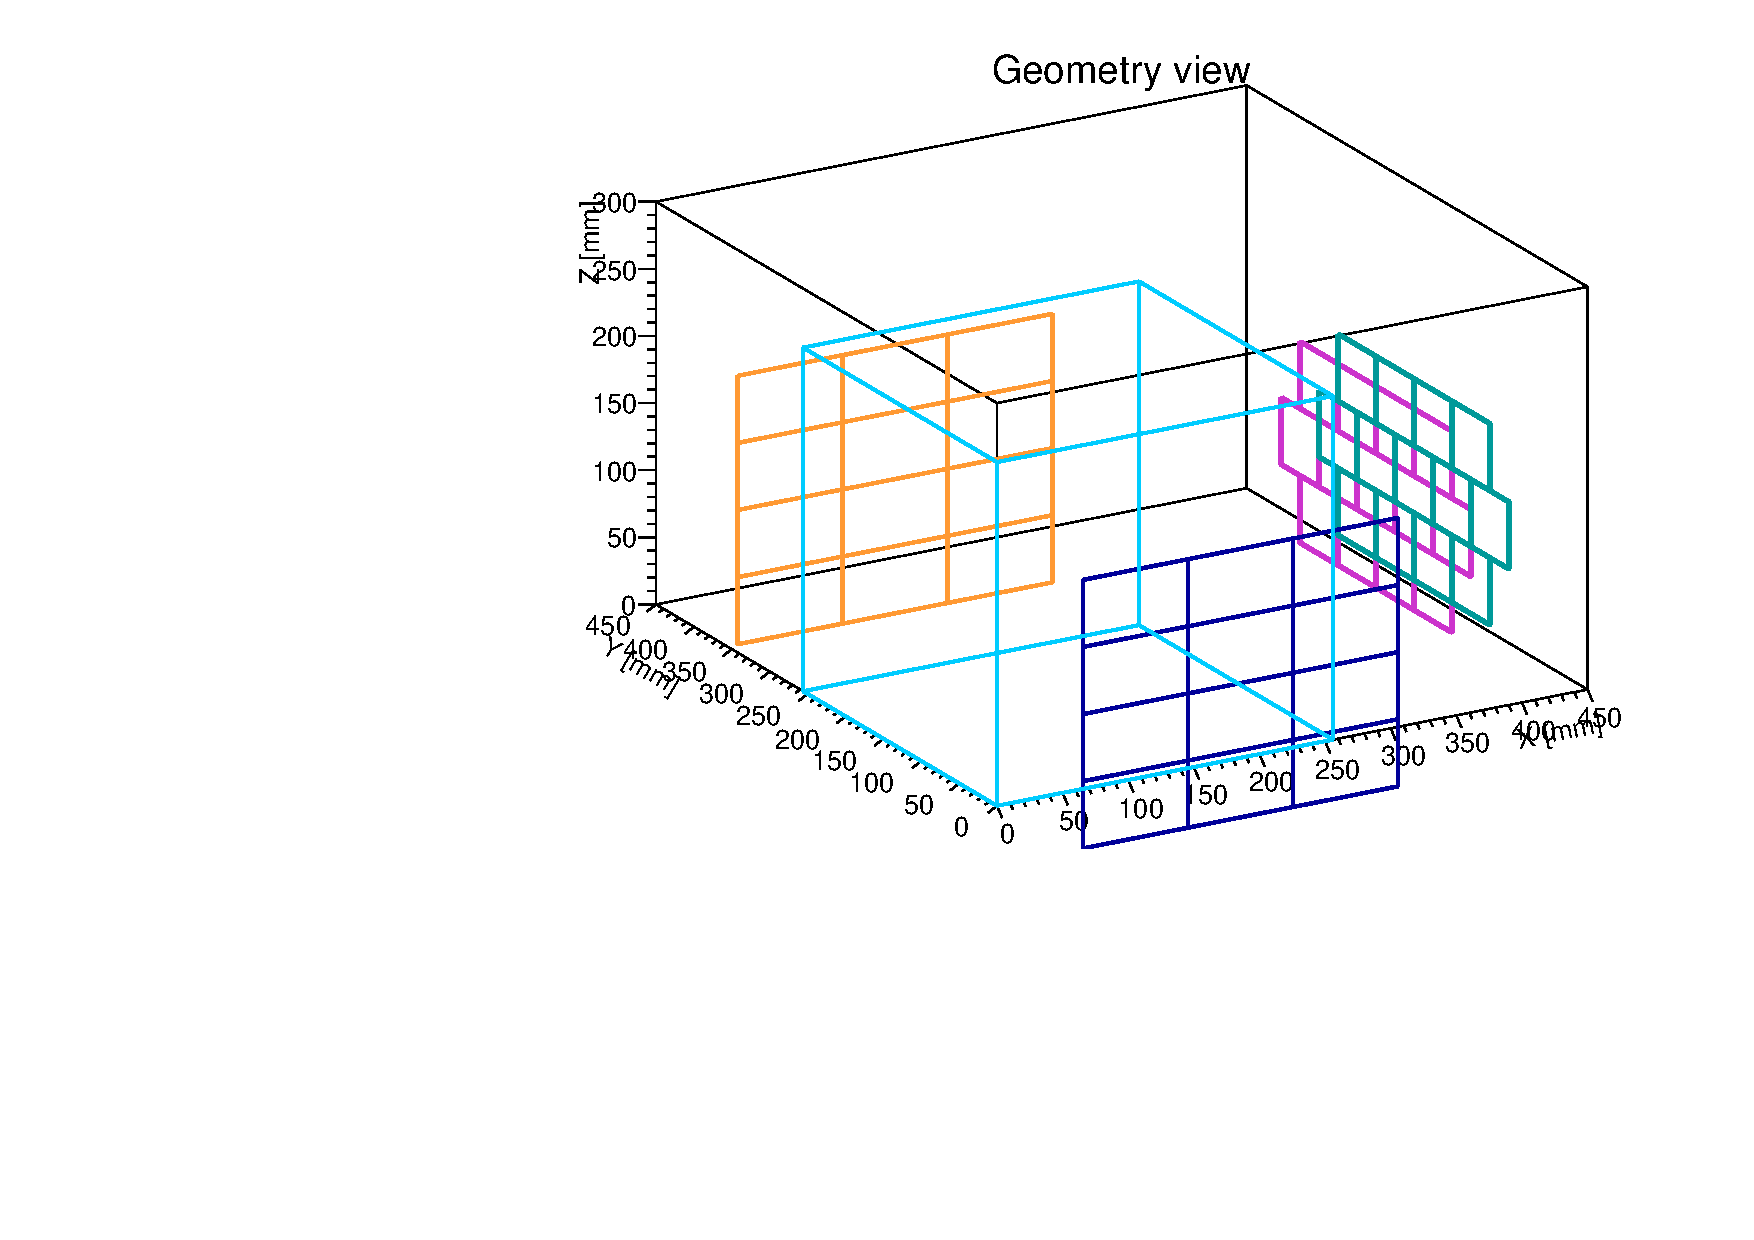
\includegraphics[width=1\linewidth]{Imagenes/Actar.pdf}
	\captionof{figure}{Dibujo de la geometría implementada en la simulación.}
	\label{Fig:Geo_Actar}
\end{minipage}


\subsection{Detectores de Silicio}

Los detectores de silicio están formados por uniones PN en los que la partícula incidente genera pares de electrones-hueco. Gracias a la presencia de una pequeña diferencia de potenicial externa introducida para que la unión esté en inversa, generando una amplia zona de vaciamiento que ocupa gran parte del detector, estos electrones derivan por acción del campo E intrínseco a la unión. Recogidos en unos conectores, la corriente eléctrica generada por ellos será directamente proporcional a su número, y este a la energía depositada por la partícula.
%, que es precisamente donde se encuentra el campo eléctrico. Es decir, aumenta el área efectiva del detector.  La intensidad de la corriente generada estará relacionada con la energía depositada.


La \textbf{resolución energética intrínseca} $R$ es una propiedad característica del dector y tiene en cuenta, entre otros factores, las fluctuaciones estadísticas en el número de partes electrón hueco generados. La resolución relacionada con el FWHM de la distribución estadística de la energía depositada en el silicio y con la energía de la propia partícula, tal que

\begin{equation}
	\text{FWHM} = R \cdot E
\end{equation}
y dado que $\sigma = 2.35 \cdot \text{FWHM} $, tenemos que la $\sigma$ de la distribución gaussiana que parece seguir la energía depositada es:

\begin{equation}
	\sigma  = \frac{R \cdot E}{2.35}
\end{equation}
La \textbf{resolución esperada} es \cite{Leo:302344}

\begin{equation}
	R = 2.35 \sqrt{\frac{0.12 w}{E}}
\end{equation}
donde \( w \) es la energía promedio para la creación de un par electrón-hueco en el semiconductor. El valor de la creación de un par electrón-hueco depende del tipo de semiconductor y de la temperatura. Por ejemplo para el silicio tenemos $w=3.62$ eV para una $T=$300K y $w=3.81$ eV si $T=77$ K, por lo que es muy importante tener controlado el ambiente. Nosotros usamos valores experimentales para obtener la $\sigma$ de la distribución \cite{Leo:302344}. En particular nosotros sabemos que para una energía de 5.5 MeV de nuestras partículas al atravesar el semiconductor contamos con una resolución de $50$ keV, tal que la $\sigma$ que vamos a usar en la simulación para parametrizar la energía depositada en los silicios viene dada por:

\begin{equation}
	\sigma = \frac{0.0213}{2.35} \sqrt{E} \ \unit{MeV} \label{Ec:03-resolucion}
\end{equation}
Podemos ver una dependencia con la raíz cuadrada de $\sigma$ con $E$, lo que nos dice que a mayor energía peor resolución. Los silicios tendrán un tamaño de $5 \times 5 \times 0.15 \ \text{cm}^{3}$, suficientemente gruesos como para parar gran parte de las partículas incidentes. Un término muy importante que se suele usar cuando hablamos de detectores de silicio es \textbf{\textit{el punch-through}}. Decimos que ocurre punch-through cuando la partícula atraviesa completamente el detector/medio sin depositar toda su energía en él.  En nuestro caso, que detectaremos tritios con los silicioes, el \textit{punch-through} sucede a partir de la energía de 24.42 MeV, que pudimos obtener a partir de una interpolación lineal de los valores experimentales \cite{ZIEGLER20101818}. 

\subsection{Cinemática} \label{Subsec:03-cinematica}

En este apartado trataremos de resolver la cinemática de la reacción de interés $^{11}\text{Li}(d,t)^{10}\text{Li}$. Resolver la cinemática basicamente implica obtener los ángulos de las partículas salientes y sus energías en función de: la energía cinética de la partícula incidente en el sistema laboratorio, que en nuestro experimento será de 7.5 MeV/A (MeV por nucleón, i.e. 82.5 MeV), el ángulo del centro de masas (que es el afectado por la sección eficaz) y la energía de excitación de la partícula $^{10}$Li.

La cinemática responde únicamente a las leyes de conservación de la energía-momento, por lo que no tendremos que tener en cuenta ni interacciones electromagnéticas ni nucleares. La sección eficaz que influye en el ángulo de salida, que encierra la física nuclear de la interacción, será discutida más adelante.

\subsubsection{Notación}
Dado que en función del sistema de referencia tendremos un valor de momento u otro, necesitaremos especificar que sistema de referencia seguimos. Usaremos las siguiente notación: $p_{1}$ es el momento en el sistema laboratorio y $p_{1}'$ es el sistema del centro de masas. En la siguiente figura presentamos un esquema de ambos sistemas de referencia, y como son las partículas para cada uno de ellos.

\begin{minipage}[t]{0.45\linewidth}
	\begin{center}
		\begin{tikzpicture}[thick,scale=0.6]
			\node (1) at (-3,0) {};
			\node (2) at (0,0) {$m_2$};
			\node (3) at (3,1) {$m_3$};
			\node (4) at (3,-1) {$m_4$};
			\node (m1) at (-1.5,0.5) {$m_1$};
			\draw[arrows={->},ultra thick] (1.east)--(2.west);
			\draw[arrows={->},ultra thick] (2.east)--(3.west);
			\draw[arrows={->},ultra thick] (2.east)--(4.west);
		\end{tikzpicture}
		\captionof{figure}{Sistema Laboratorio}
	\end{center}
\end{minipage}
\hfill
\begin{minipage}[t]{0.45\linewidth}
	\begin{center}
		\begin{tikzpicture}[thick,scale=0.6]
			\node (1) at (-3.5,0) {};
			\node (2) at (3.5,0) {};
			\node (3) at (1.8,2.8) {};
			\node (4) at (-1.8,-2.8) {};
			\draw[arrows={->},ultra thick] (1.east)--(-0.1,0)  ;
			\draw[arrows={->},ultra thick] (2.west)--(0.1,0)  ;
			\draw[arrows={->},ultra thick] (0.1,0.1)--(3.south west)  ;
			\draw[arrows={->},ultra thick] (-0.1,-0.1)--(4.north east)  ;

			\node (m1) at (-1.75,0.3) {$m_1$};
			\node (m2) at (1.75,0.3) {$m_2$};
			\node (m3) at (2.3,1.8) {$m_3$};
			\node (m4) at (-1.8,-1.8) {$m_4$};
		\end{tikzpicture}
		\captionof{figure}{Sistema Centro de Masas}
	\end{center}
\end{minipage}

\subsubsection{Cálculo de los ángulos y energías}
En este apartado trataremos de obtener los ángulos de salida de las partículas 3 y 4 (y sus energías) en función de las variables conocidas: energía cinética y masas de las partículas. Para esto necesitaremos calcular las energías de las partículas en el sistema centro de masas, ya que las relaciones de conservación de la energía es mucho mas sencilla en este sistema referencial. Luego podremos recuperarlas usando la \textit{transformada de Lorentz}.

Como podemos ver en las figuras, en el sistema laboratorio la partícula 1 está en movimiento mientras que la partícula 2 está en reposo. Recordamos que la \textbf{masa de una partícula excitada} $i$ viene dada por
\begin{equation}
    m_i = m_{i,g.s} + E_{ex}
\end{equation}
donde $E_{ex}$ es la energía de excitación y $m_{i,g.s}$ la energía en su estado fundamental. Esto nos lleva a que sus momentos, en el sistema de referencia del laboratorio:

\begin{eqnarray}
	P_1 = (E_1/c,\pn_1) & \quad P_2 = (m_2c,0) \\
	P_3 = (E_3/c,\pn_3) & \quad P_4 = (E_4/c,\pn_4)
\end{eqnarray}
Por otro lado, los momentos en el sistema de referencia del centro de masas vendrán dados por

\begin{eqnarray}
	P_1' = (E_1'/c,\pn_1') \quad P_2 = (E_2'/c,-\pn_1') \\
	P_3' = (E_3'/c,\pn_3') \quad P_4 = (E_4'/c,-\pn_3')
\end{eqnarray}
Asumiremos que la partícula 1 incidente se mueve únicamente en el eje $x$ tal que $\pn_1=(p_1,0,0)$. En ese caso el sistema centro de masas se moverá respecto al sistema laboratorio en el eje $x$, por lo que habrá que aplicar la transformaciones de Lorentz, siendo válidas para \textit{cualquier cuadrimomento}. Definimos las energías totales como $E_{tot}=E_1+E_2$ y como  $E_{tot}'=E_1'+E_2'$, siendo esta última la \textit{energía del centro de masas}, que verifica que
\begin{equation}
	E_{tot}' \equiv E_{CM} = E_{tot}^2 - c^2p_1^2 \label{Ec:18}
\end{equation}
Tanto $E_{tot}$ como $E_{tot}'$ son variables conocidas. Nos interesa calcular las energías $E_3'$ y $E_4'$, que usando la transformación de Lorentz nos servirán para estudiar las energías $E_3$ y $E_4$, así como los momentos.  Así pues:
\begin{eqnarray}
	E_3 ' & = & \frac{1}{2} \left( E_{tot}' + \frac{m_3^2c^4- m_4^2c_4}{E_{tot}'} \right) 
\end{eqnarray}
A partir de estos valores de $E_3'$ podemos calcular el valor de los momentos $p_3'$  (en módulo). Podemos suponer sin ningún tipo de problema que la coordenada $x$ de los momentos vienen dadas por


\begin{eqnarray}
	p_{3x}' = p_3' \cos (\theta_3') 
\end{eqnarray}

de este modo podemos aplicar las transformaciones de Lorentz para hallar los valores del $\cos (\theta_3)$ y $\cos (\theta_4)$. Así:

\begin{minipage}{0.48\linewidth}
\begin{equation}
	p_3 \cos (\theta_3) = \gamma (p_3' \cos (\theta_3')+\beta E_3'/c)
\end{equation}
despejando $\cos (\theta)$ obtenemos:
\begin{equation}
	\cos (\theta_3) = \frac{\gamma}{p_3} (p_3' \cos (\theta_3')+\beta E_3'/c)
\end{equation}
El cálculo de $p_4$ es completamente análogo. En la siguiente \cref{Fig:04-Kin} podemos ver la dependencia entre el ángulo $\theta_3$ y $\theta_4$ y la energía cinética de salida, en la que podemos ver una función que las relaciona inequívocamente. Podemos observar que a medida que aumentamos la energía de excitación se comprime el ángulo y el rango de las energías cinéticas que abarca la cinemática. Cabe destacar que en la figura usamos una energía de excitación que no se corresponde con una excitación física del \litioDiez, buscando que se vea el efecto de la energía de excitación en al cinemática. 
\end{minipage}
\hfill 
\begin{minipage}{0.48\linewidth} \centering
	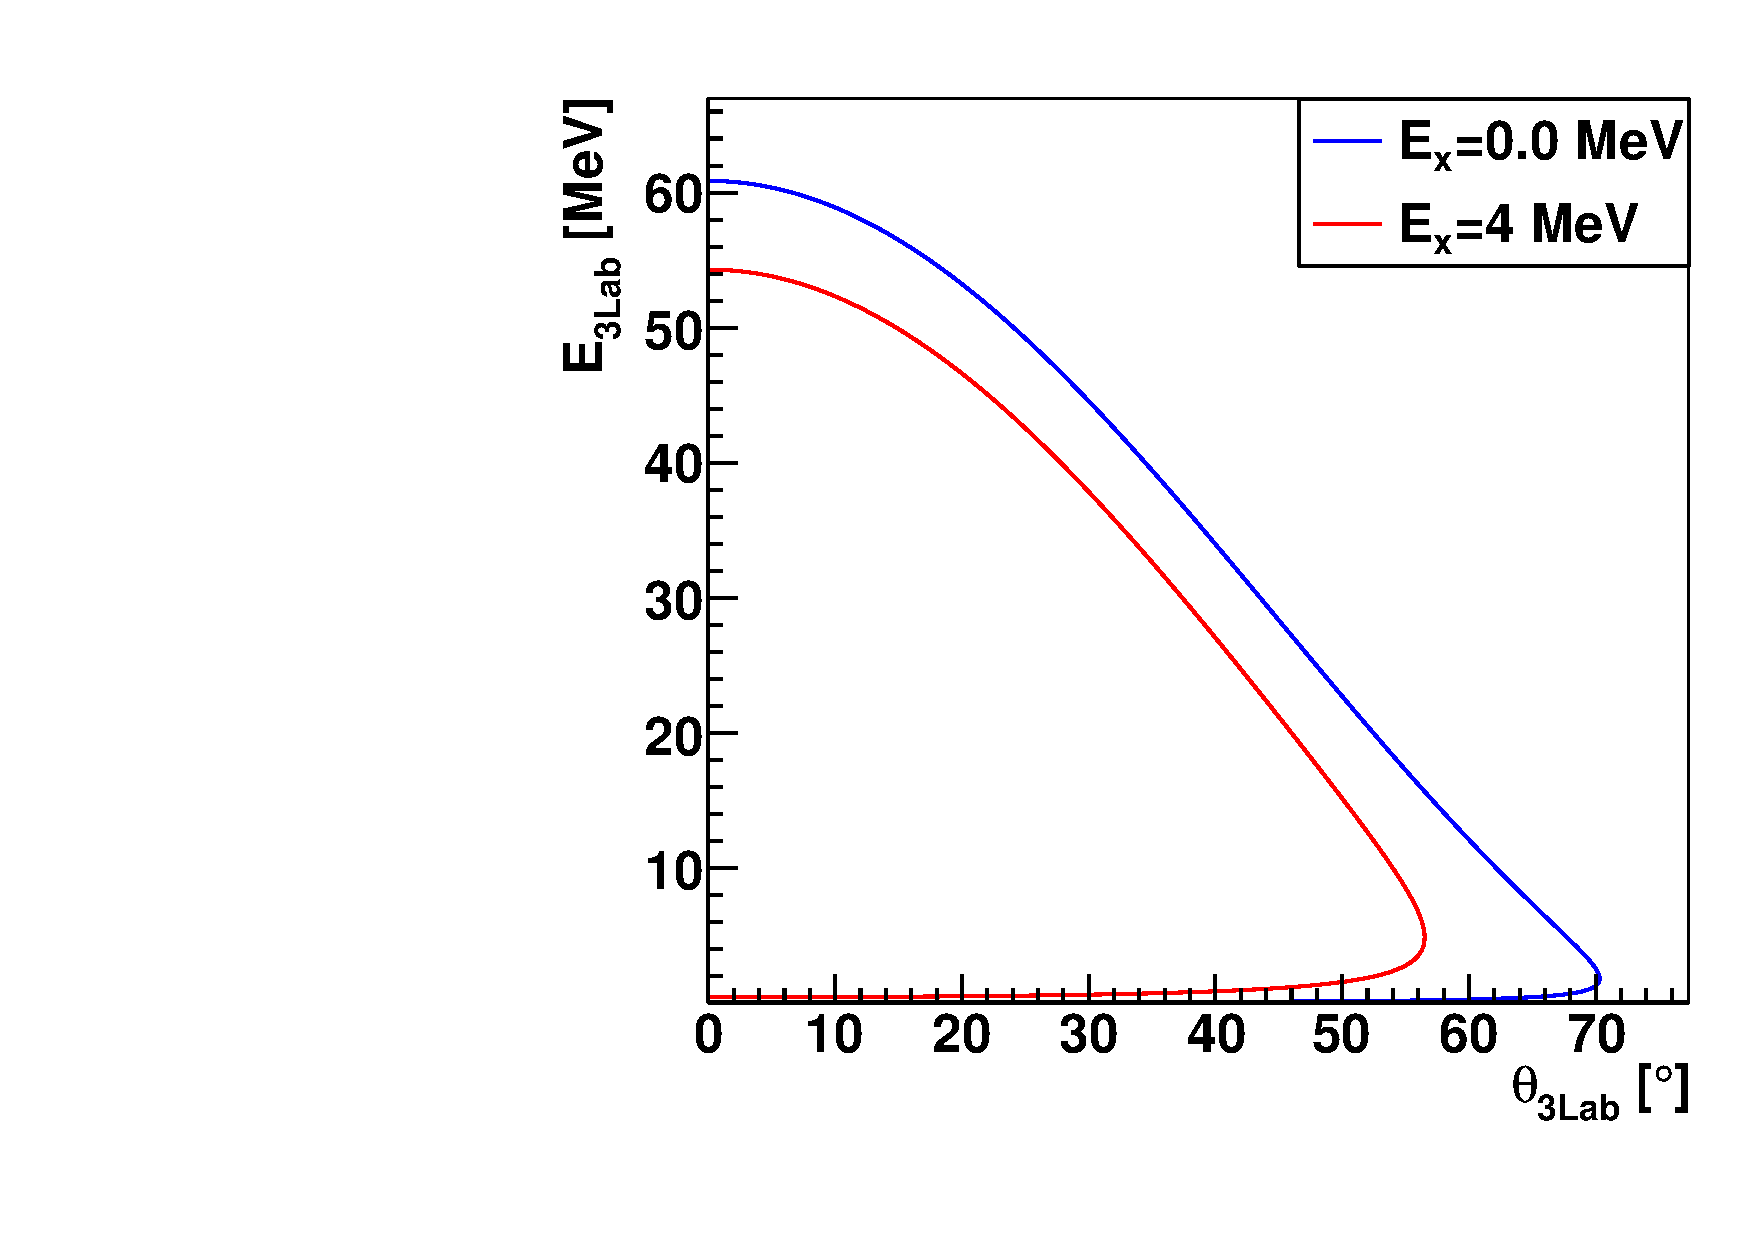
\includegraphics[width=1\linewidth]{Imagenes/Cinematica.pdf}
	\captionof{figure}{Cinemática de la reacción $^{11}\text{Li}(d,t)^{10}\text{Li}$ para energía incidente de $7.5$ MeV/A, donde se muestra la energía cinética del tritio (izquierda) frente su ángulo de salida.}

	\label{Fig:04-Kin}
\end{minipage}


\subsection{Pérdidas de energía en la materia}

Las pérdidas de energía por culpa de la interacción con la materia son sumamente importantes en el estudio de cualquier detector, ya que tendrán que ser tenidas en cuenta a la hora de recuperar la energía en el laboratorio de las partículas ligeras. La mejor manera de caracterizar la pérdida de energía de una partícula en un medio viene dada por la \textbf{ecuación de Bethe-Bloch} (en nuestro caso usarmeos la aproximación no relativista), que nos dice que el poder de frenado lineal $S$, definido como la pérdida de energía de la partícula dividida por la longitud diferencial de la trayectoria  \cite{Knoll:1300754}

\begin{equation}
	S = - \frac{dE}{dx} \simeq \frac{4 \pi e^4}{m_e} \left( \rho \frac{N_A}{M} \right) \frac{z^2 Z}{v^2} \ln \left( \frac{2 m_e v^2}{I} \right)
\end{equation}
donde $z$ es el número atómico incidente, $Z$ la de la partícula absorbente, $v$ la velocidad de la partícula incidente, $N_A$ el número de avogadro, $M$ la masa atómica del gas, $\rho$ su densidad (por lo que dependerá de la presión, un parámetro importante) e $I$  representa el potencial promedio de excitación e ionización del absorbente. Se trata como un parámetro determinado experimentalmente para cada elemento cuyo orden de magnitud se sitúa alrededor de unas decenas de eV.

Entrando ya en nuestro detector, mientras que para describir la interacción partículas-silicio esta ecuación es suficiente, ACTAR TPC contendrá  una mezcla de gases, por lo que la ecuación de la pérdida no será exactamente la anterior, si no que responderá a la \textbf{regla de Bragg-Kleeman} \cite{Knoll:1300754}
\begin{equation}
	\frac{1}{N_c} \left( \frac{dE}{dx} \right)_c = \sum_i W_i \, \frac{1}{N_i} \left( \frac{dE}{dx} \right)_i
\end{equation}
siendo $W_i$ el peso del gas $i$ y $N_i$ la densidad atómica tal que $N_i = \rho N_A	/ M_i$.

\begin{minipage}{0.48 \linewidth}
El valor de \( -dE/dx \) a lo largo de la trayectoria de una partícula también se llama su \textit{pérdida específica de energía}, una ``tasa'' de pérdida de energía. En realidad esta ecuación nos habla de un promedio, ya que la interacción partícula-partícula es un fenómeno estadístico que es muy poco probable. Debido precisamente a esta baja probabilidad, cada partícula, pese a que tenga una energía inicial idéntica, recorrerá una distancia diferente (o lo que es lo mismo, para un mismo rango recorrido dos partícuals no tendrán porque tener la misma enerǵia inicial). Estas fluctuaciones debido a su naturaleza estocástica en la energía cinética las llamamos \textbf{\textit{straggling}}. Este \textit{straggling} nos lleva a un error indefectible en la recuperación de la energía cinética experimental y simulada cuando aplicamos esta ecuación. 

\end{minipage}
\hfill
\begin{minipage}{0.48\linewidth}
    \centering
    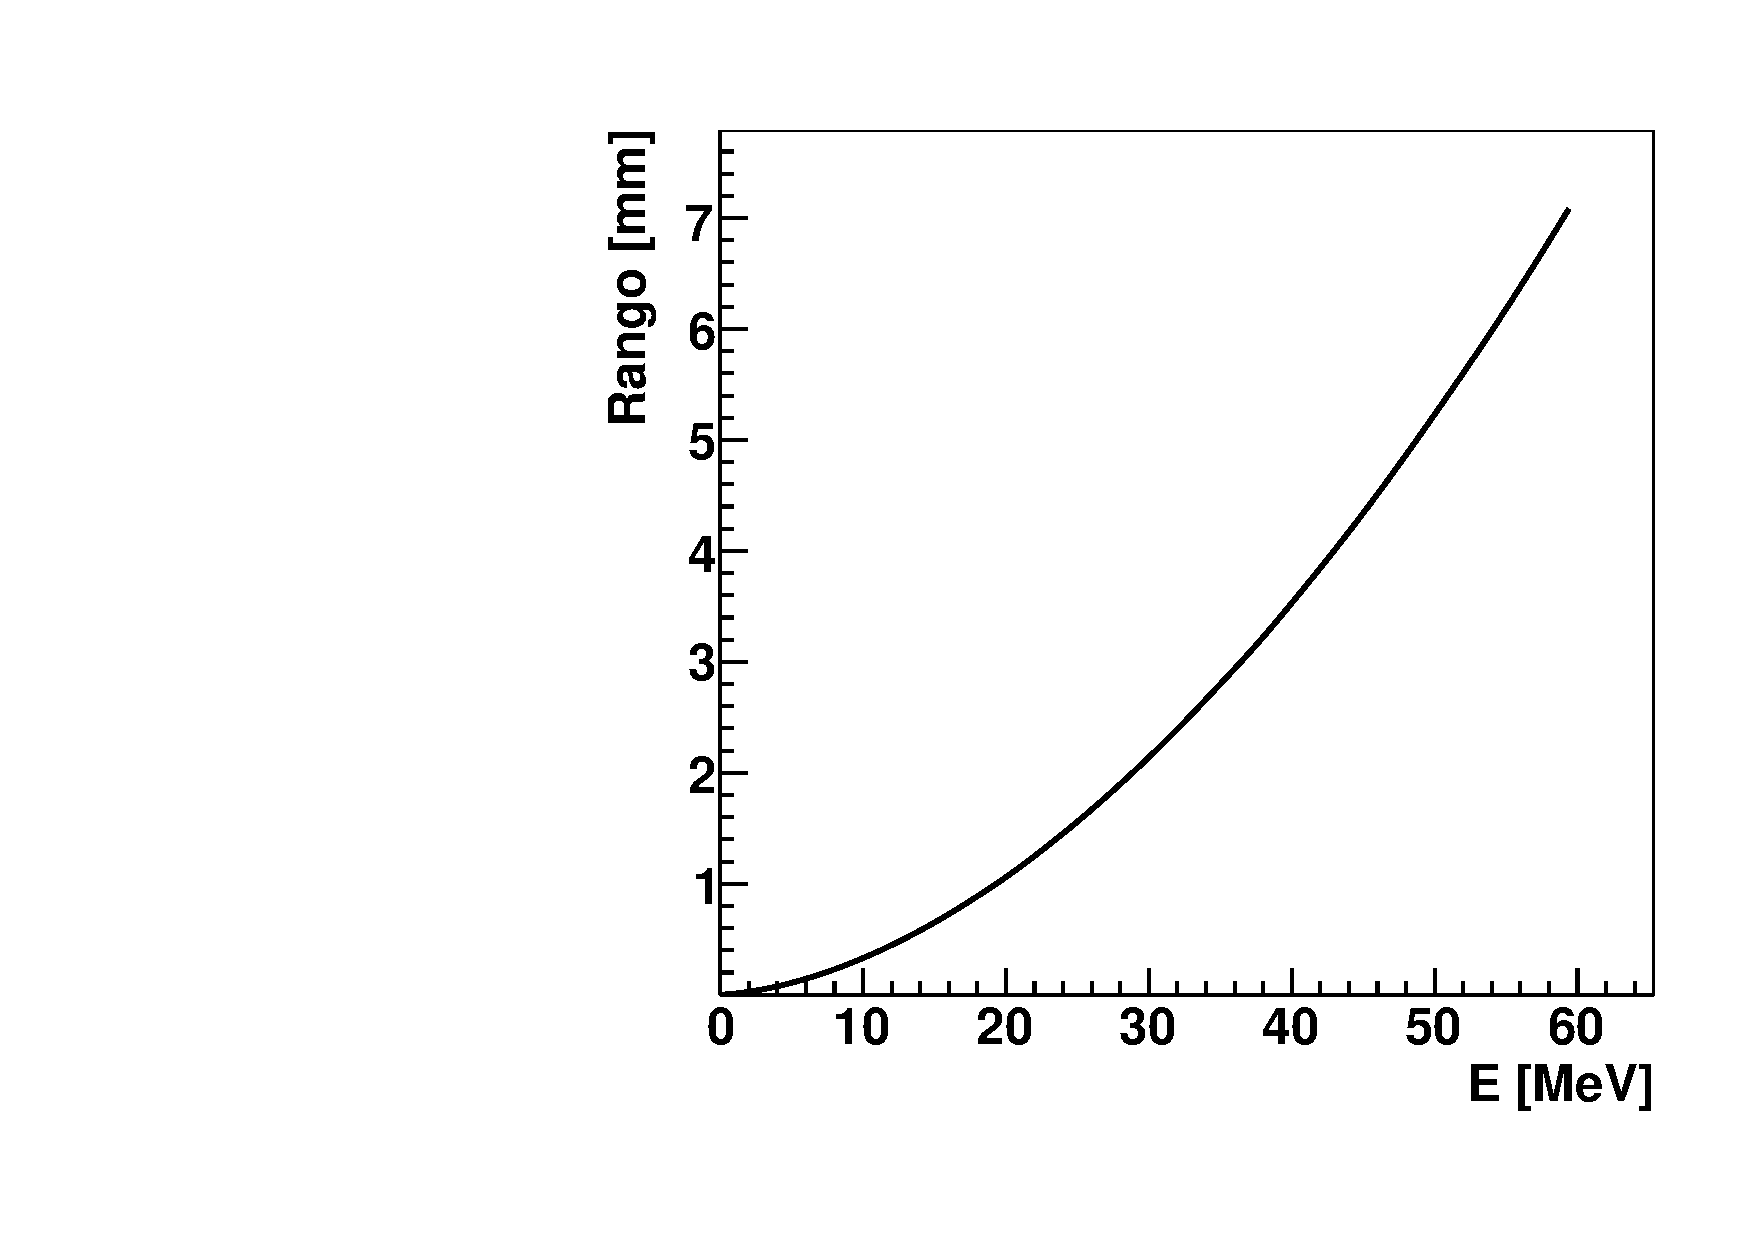
\includegraphics[width=1\linewidth]{Imagenes/RangoEnergiaTeo.pdf}
    \captionof{figure}{Rango para cada energía para el tritio en el gas.}
    \label{Fig:03-RangoTheta}
\end{minipage}

El \textbf{rango} se define como la distancia para la cual las partículas se paran en el medio. El rango depende de la energía inicial, por lo que existe una relación uno a uno del rango y la energía inicial, tal y como podemos ver en la \cref{Fig:03-RangoTheta}. Además el fenómeno estadístico nos dice que cada rango tendrá una distribución de probabilidad única (i.e., un \textit{straggling}). Así pues, conociendo el vértice de interacción y el momento en el que se frena, podremos obtener el rango de la partícula, que al tener una relación uno a uno con la energía podremos usar para extraer información de la energía de la partícula en el vértice.  


\subsection{Resolución angular}

Gracias a la TPC podemos reconstruir la traza del tritio que nos da información acerca del ángulo $\theta_{lab}$ de las partículas resultantes de la reacción. Experimentalmente esta información viene en forma de una nuble de puntos que hay que clusterizar y ajustar (mediante una regresión lineal 3D), y una vez conocida da dirección del haz, $\theta$ se obtiene como el ángulo entre ambas direcciones. En experimentos previos \cite{MAUSS2019498} se ha visto que la resolución en esta variable, ligada al tamaño finito de los \textit{pads}, se sitúa en $1^{\circ}$ FWHM. Como veremos más adelante, este factor será el dominante entre nuestras incertidumbres.

%que podremos obtener $\theta$ sabiendo la dirección incidente. La distribución de cada medida de $\theta_{lab}$ sería una gaussiana con FWHM = 1$^{\circ}$, que será, tal y como veremos, el factor que generá mas anchura $\sigma$ en las distribuciones de energía. Este valor fue obtenido en experimentos previos \cite{MAUSS2019498}.

\subsection{Sección eficaz}

La sección eficaz diferencial nos da información acerca de la distribución de probabilidad de que una partícula saliente tenga una dirección respecto el haz inicial específico. Se define como el área efectiva por unidad de ángulo sólido $\D\Omega(\theta,\phi)$ que caracteriza la dispersión en cada dirección. Matemáticamente se expresa como
\begin{equation}
\frac{\D\sigma}{\D\Omega(\theta,\phi)},
\end{equation}
donde $\D\sigma$ es la sección eficaz para partículas dispersadas dentro de un elemento de ángulo sólido $\D\Omega(\theta,\phi)$. Por otro lado la sección eficaz global nos habla de la probabilidad de interacción de dos partículas en un canal determinado (elástico, inelástico...) modelado a través de una superficie efectiva, lo que nos viene a decir que contiene información física sobre el espín, paridad... ya que todos estos factores están relacionados con la interacción entre las partículas.

Esta sección eficaz diferencial es diferente para cada excitación, la de 0.0 MeV (\textit{ground-state}) y anchura 0.1 MeV asociado con el orbital $2s_{1/2}$ y la de 0.2 MeV y anchura 0.2 MeV asociada con el orbital $1p_{1/2}$, tal y como podemos ver en la \cref{Fig:04-seccion_eficaz}, por lo que la distribución a \textit{samplear} en $\theta_{\text{CM}}$ dependerá del estado a considerar. 

\begin{center}
	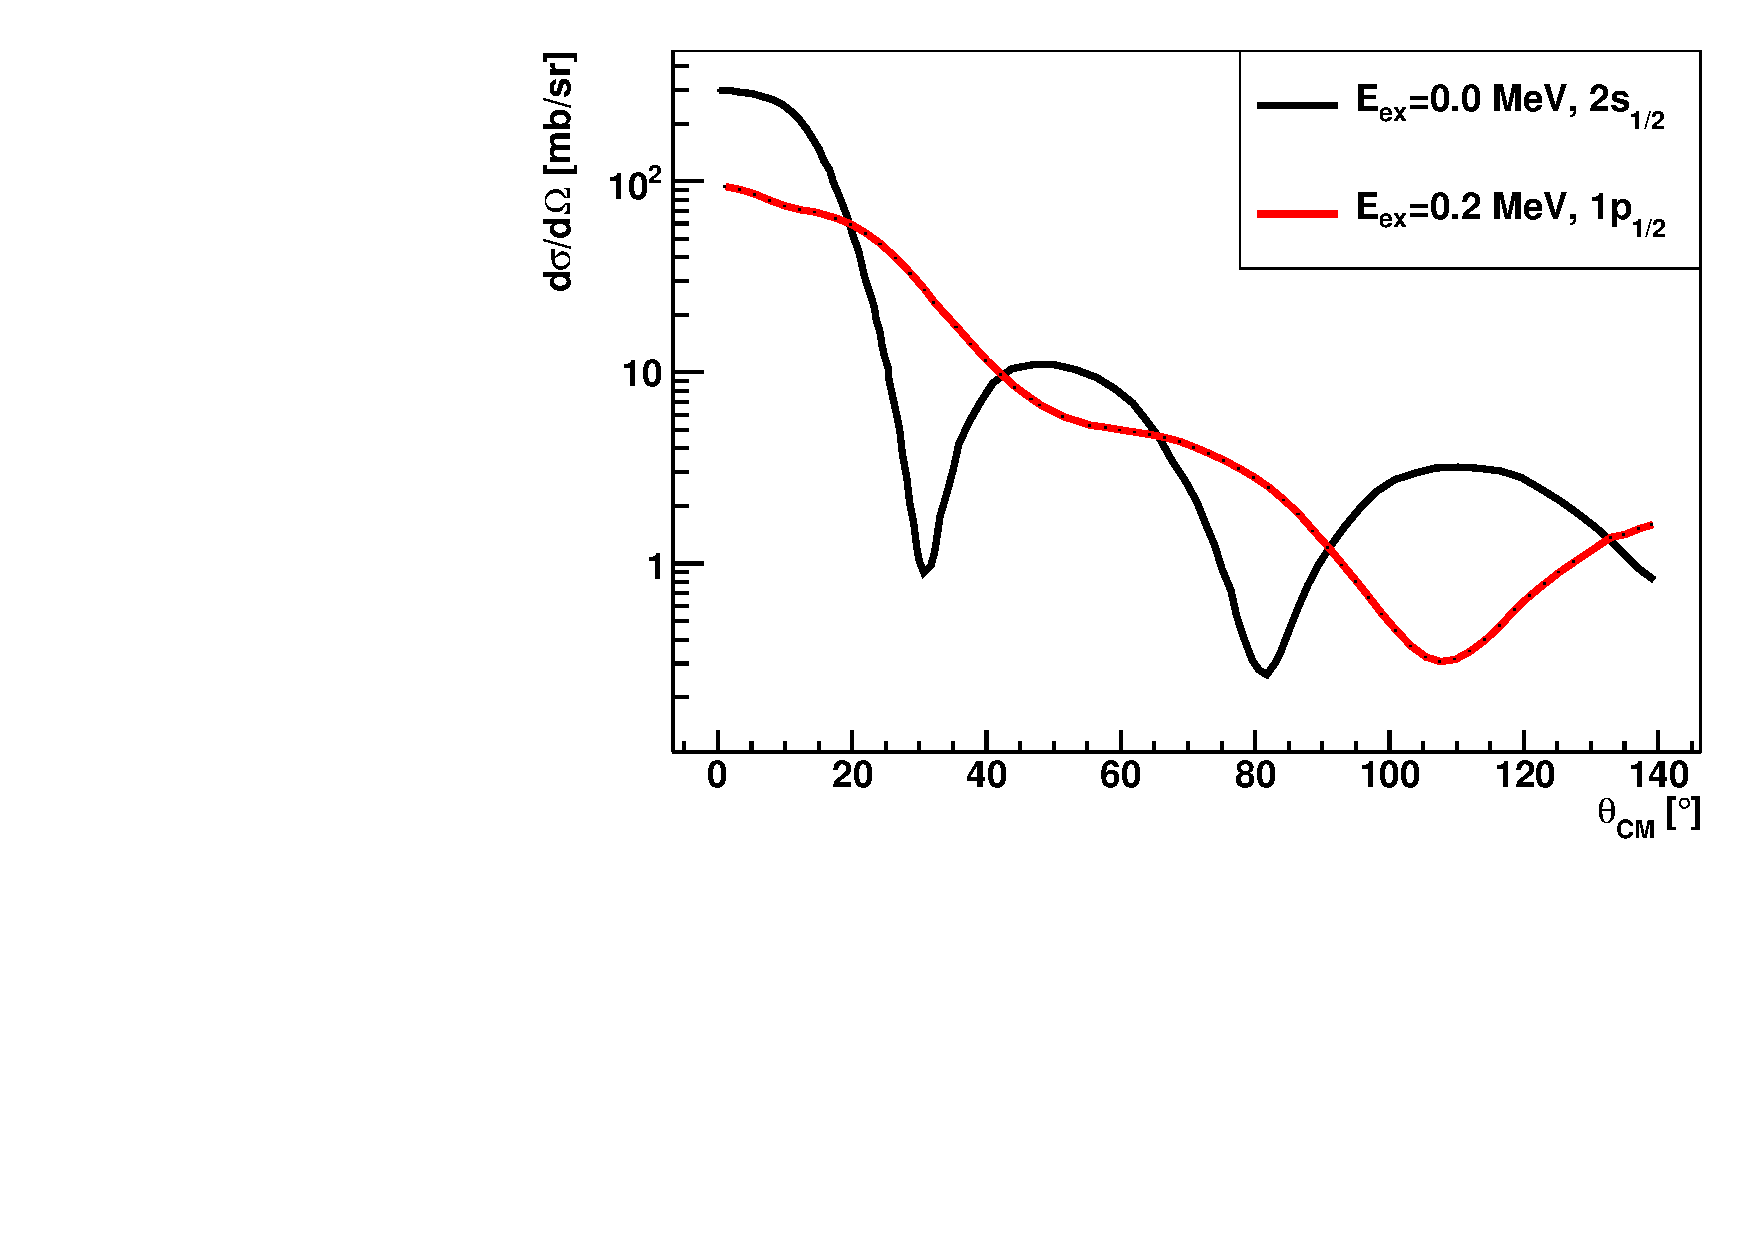
\includegraphics[width=0.7\linewidth]{Imagenes/Seccion_Eficaz.pdf}
	\captionof{figure}{Sección eficaz teórica que usaremos para ambas excitaciones.}
	\label{Fig:04-seccion_eficaz}
\end{center}


\subsection{Estadística real vs simulada}

En nuestra simulación emitimos una cantidad de partículas a nuestra elección, suficiente para tener una buena estadística y un costo computacional moderado. En el experimento no todas las partículas del \textit{beam} interaccionan con el gas de la TPC según la reacción de interés $^{11} \text{Li}(d,t)^{10}\text{Li}$, ya que se trata de un fenómeno probabilístico determinado por la sección eficaz; además, no todos los eventos son detectados, lo que afecta la eficiencia del sistema (el cociente entre eventos detectados y eventos que realmente ocurren es la eficiencia). Tenemos, de alguna forma, que obtener una relación entre el número de cuentas procedentes del experimento con el que nos queremos comparar y la simulación, de tal modo que podamos relacionar los resultados entre ambas. Así:

\begin{equation}
	N_{\text{eventos}}  = N_{\text{beam}} \cdot N_{\text{targets}} \cdot \sigma \cdot \epsilon \label{Ec:3.21}
\end{equation}
donde $\sigma$ es la sección eficaz total integrada en todo el ángulo solido y $\epsilon$ es la eficiencia. 

Por otro lado, para la simulación todas las partículas de entrada experimentarán dicha reacción con un 100\% de probabilidad, teniendo en cuenta la sección eficaz más como una distribución del ángulo de salida que como un factor de probabilidad de  que suceda la reacción. En la simulación el número de eventos es, denotándolo con una prima:

\begin{equation}
	N'_{\text{eventos}} = N_{\text{iter}} \cdot \epsilon
\end{equation}
siendo $\epsilon$ la misma eficiencia que la de la \cref{Ec:3.21}. Lógicamente en ambos casos tendremos la misma eficiencia ya que los factores geométricos y de interacción radiación-materia están incluidos en la simulación.


Para recuperar los eventos reales tendremos que multiplicar por un factor $\alpha$ calculado a través de la división de los valores anteriores: 
\begin{equation}
	\alpha=\frac{N_{\text{eventos}}}{N_ {\text{eventos}'}} = \frac{N_{\text{beam}} \cdot N_{\text{targets}} \cdot \sigma}{N_{\text{iter}}}
\end{equation}
Para poder relacionar correctamente un histograma de la simulación y el histograma real bastará con multiplicarla por este factor $\alpha$, tal que:

\begin{equation}
	\text{Histograma real} =  \alpha \cdot \text{Histograma simulado }
\end{equation}
Ahora tenemos que calcular de alguna forma este $\alpha$. Primero debemos de hacer la integral de $\sigma$, obteniendo 

\begin{table}[H] \centering
	\begin{tabular}{llllllll} \hline
\toprule 
 & $\sigma(0.0)$ [mb]  &  $\sigma(0.20)$ [mb]  \\ \midrule 
Trapecio & $\num{108.6774}$ & $\num{83.6741}$\\ 
Simpson & $\num{108.6895}$ & $\num{83.6919}$\\ 
 \bottomrule 
\end{tabular}

	\caption{Valores de la sección eficaz total para ambas excitaciones.}
\end{table}
Los parámetros que  usaremos tendrán en cuente un haz de $^{11}$Li con una intensidad de 3000 partículas por segundo que durará 6 días, por lo que
\begin{equation}
	N_{\text{beam}} = \num{3.1e+9} \ \text{partículas}
\end{equation}
Para calcular el número de partículas del gas en la dirección incidente usamos:
\begin{equation}
	N_{\text{targets}} = f_{d}N_{\text{gas}} l_x
\end{equation}
donde hemos usado que la fracción de deuterio es 78.26\%, la densidad del gas es $N_{\text{gas}}=\num{4.99E+19}$ átomos/cm$^{3}$ y que $l_x=25.5$ cm \cite{ZIEGLER20101818}. Empleando $N_{iter}=10^6$, podemos obtener un valor $\alpha$:
\begin{equation}
	\alpha (0.0)= {0.336920} \qquad  
\alpha (0.2)={0.259406}

\end{equation}

\section{Simulación }
\section{Análisis de los resultados}

En esta sección vamos a analizar los resultados obtenidos en la simulación, centrándonos principalmente en las diferentes anchuras de la energía de excitación recostruida. Dado que tendremos dos anchuras, en función de la energía de excitación vamos a usar la notación $\sigma(E^*)$ como anchura del ajuste gaussiano a la distribución de energía de excitación recostruida para $E^*$.  

\subsection{Recostrucción sin fuentes de incertidumbre}

En primer lugar vamos a analizar la recostrucción de la energía de excitación sin considerar ninguna fuente de incertidumbre de las aquí modeladas, que como ya mencionamos son el sttragling, la dispersión angular y la resolución de los silicios. Como podemos ver en la imagen \cref{Fig:05-RecExcIdx3}, obtenemos prácticamente una distribución Briet-Wigner, con 

\begin{equation}
    \sigma_{0} (0) = \num{0.001363305730(0.0000960943)} \text{ MeV} \quad 
    \sigma_{0} (0.2) = \num{0.011362236853(0.0034089820)} \text{ MeV}
\end{equation} 
el origen de esta $\sigma$ se puede deber al cálculo numérico del ordenador, ya que entre interacción e interacción se pierden dígitos, posibles errores sistemáticos en la simulación, e incluso errores en la generación de las distribuciones de los parámetros iniciales (energía de excitación, punto de interacción...). En cualquier caso, un análisis máx exahustivo del error permitiría obtener un origen claro de esta $\sigma$, y sería una buena práctica para futuras simulaciones.

\vspace*{-0.25cm}
\begin{figure}[H]
    \centering
    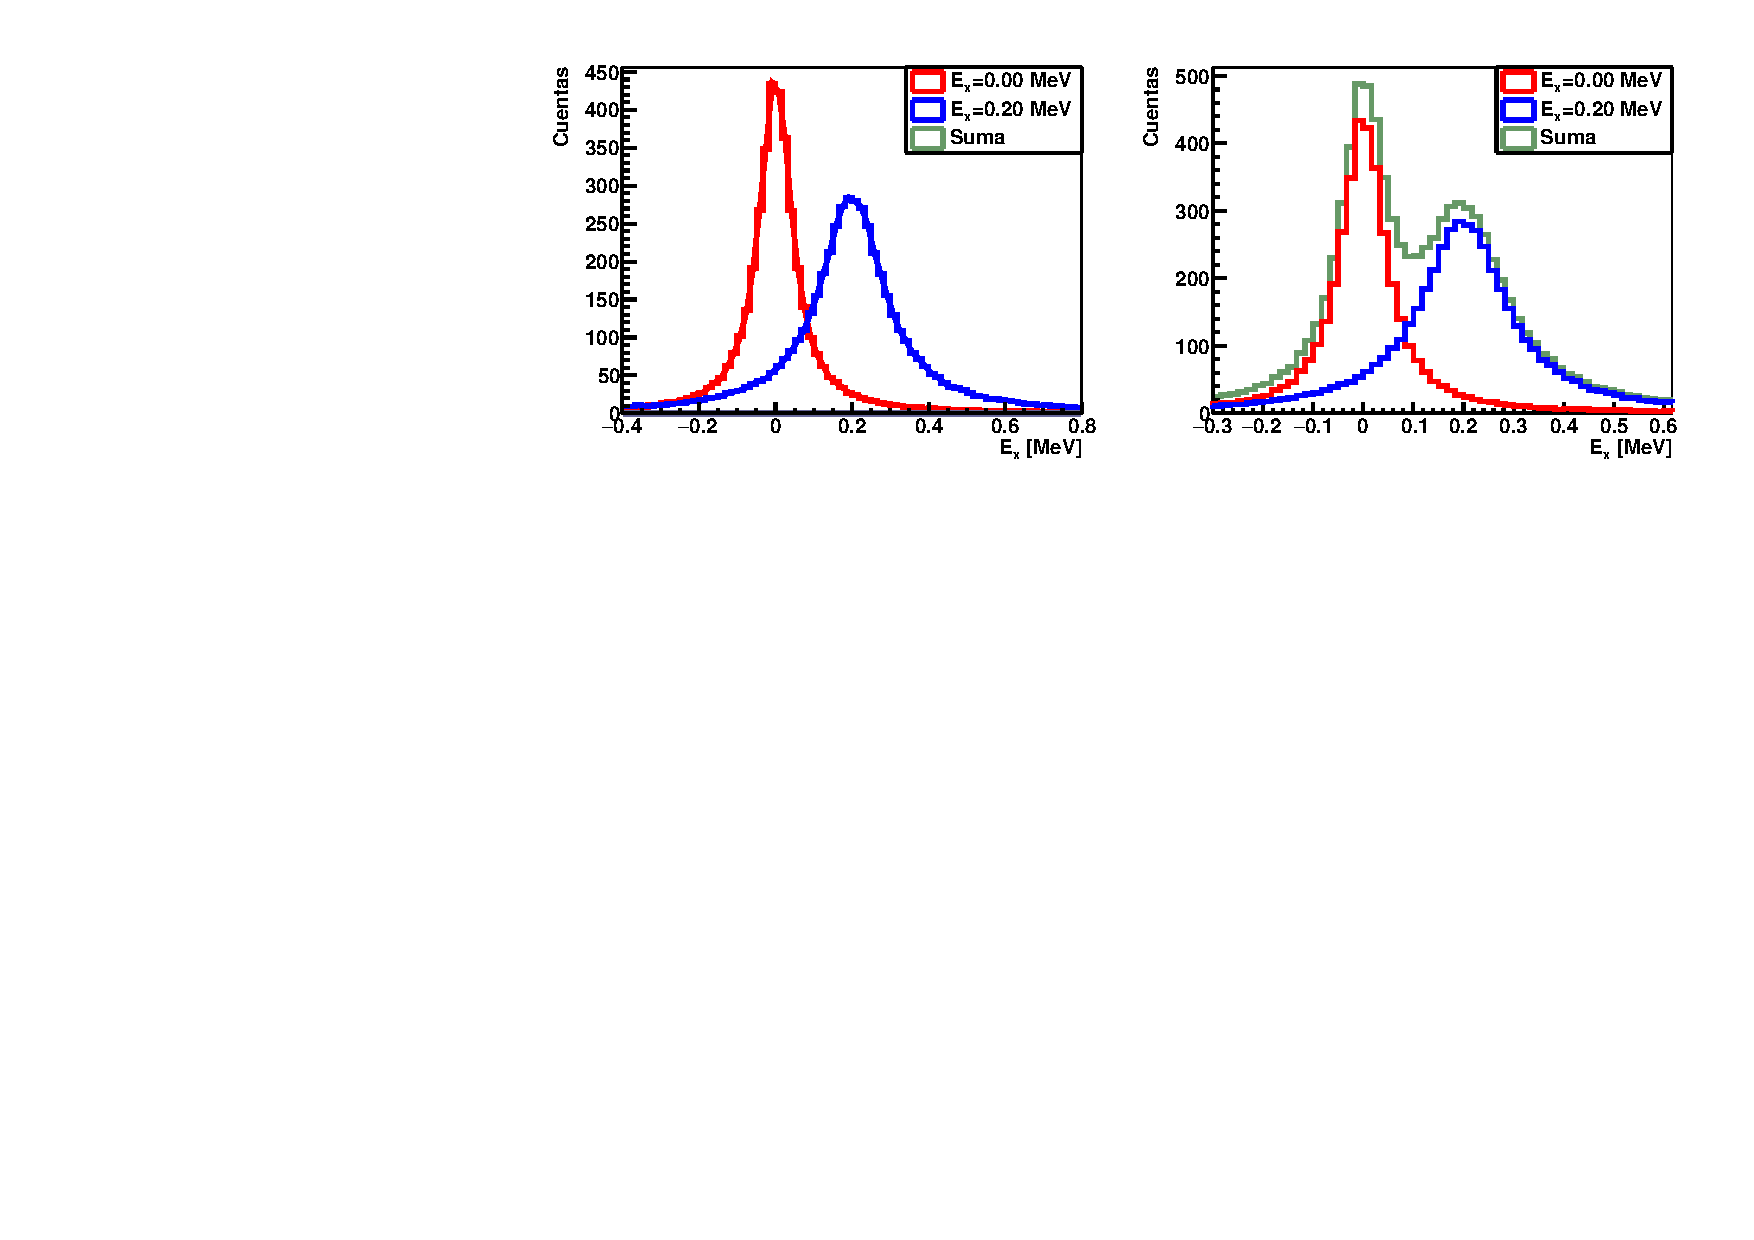
\includegraphics[width=1\textwidth]{Imagenes/Rec_incIdx3_single.pdf}
    \caption{Energía de excitación sin incertidumbre.}
    \label{Fig:05-RecExcIdx3}
\end{figure}

En cualquier caso, podemos ver claramente que la anchura intríseca de los estados del litio 10 ya produce un efecto de superposición de picos que dificultará el tratamiendo de datos experimentales, incluso reduciendo errores sistemáticos y estadísticos.

Cada una de las $\sigma$ obtenidas estarán afectadas por este error, tal que en realidad la $\sigma$ que podemos inferir de la simulación será:
\begin{equation}
    \sigma_{real}^2 = \sigma_{obtenida}^2 - \sigma_{0}^2
\end{equation}
Aunque como podemos ver en  \cref{Tab:05-ExcRec} la $\sigma_{0}$ es muy pequeña comparándola con lo obtenido en los otras simulaciones, por lo que podemos considerar que la $\sigma$ obtenida es prácticamente la real. 



\subsection{Recostrucción solo con straggling y resolución del silicio}

En este apartado vamos a analizar la recostrucción de la energía de excitación considerando únicamente el straggling y la resolución del silicio, es decir, $\sigma_{straggling}$ y $\sigma_{sil}$, que se pueden considerar como

\begin{equation}
    \sigma_{str}^2 = \sigma_{straggling}^2 + \sigma_{sil}^2
\end{equation}
Como podemos ver en la imagen \cref{Fig:05-RecExcIdx1}, ahora ya vemos más superposición en los picos, tal que en la suma de ambos histogramas no diferenciamos dos picos como si teníamos en el caso anterior. Curiosamente, es el efecto de la incertidumbre el que ahora hace que el pico más ancho sea el pico del estado fundamental y no del estado excitado. Todo esto se refleja en los resultados obtenidos: 

\begin{equation}
    \sigma_{str} (0) = \num{0.086197097183(0.0004708945)} \text{ MeV} \quad 
    \sigma_{str} (0.2) = \num{0.065691148826(0.0011537355)} \text{ MeV}
\end{equation} 
Este comportamiento podría parecer, en un principio, carente de sentido, y más cuando tenemos en cuenta que para un mismo ángulo la energía en el caso de la interacción con excitación tiene menos energía \cref{Fig:04-Kin}, lo que hace que la tasa de interacción con el gas de la cámara sea mayor y por tanto mayor debería ser el sttragling del gas. Sin embargo es precisamente por esto por lo que ocurre: pese a que lo que acabamos de decir es cierto, si nos fijamos en las secciones eficaces \cref{Fig:04-seccion_eficaz} y en la cinemática sampleada \cref{Fig:04-kinSampled0} y \cref{Fig:04-kinSampled2}, vamos claramente que para $E^*=0.0$ existe una mayor cantidad de estados con energías pequeñas, por lo que en realidad sufrirán más sttragling (en promedio) los tritios procedentes de interacciones en los que participa el estado fundamental. 


\vspace*{-0.55cm}
\begin{figure}[H]
    \centering
    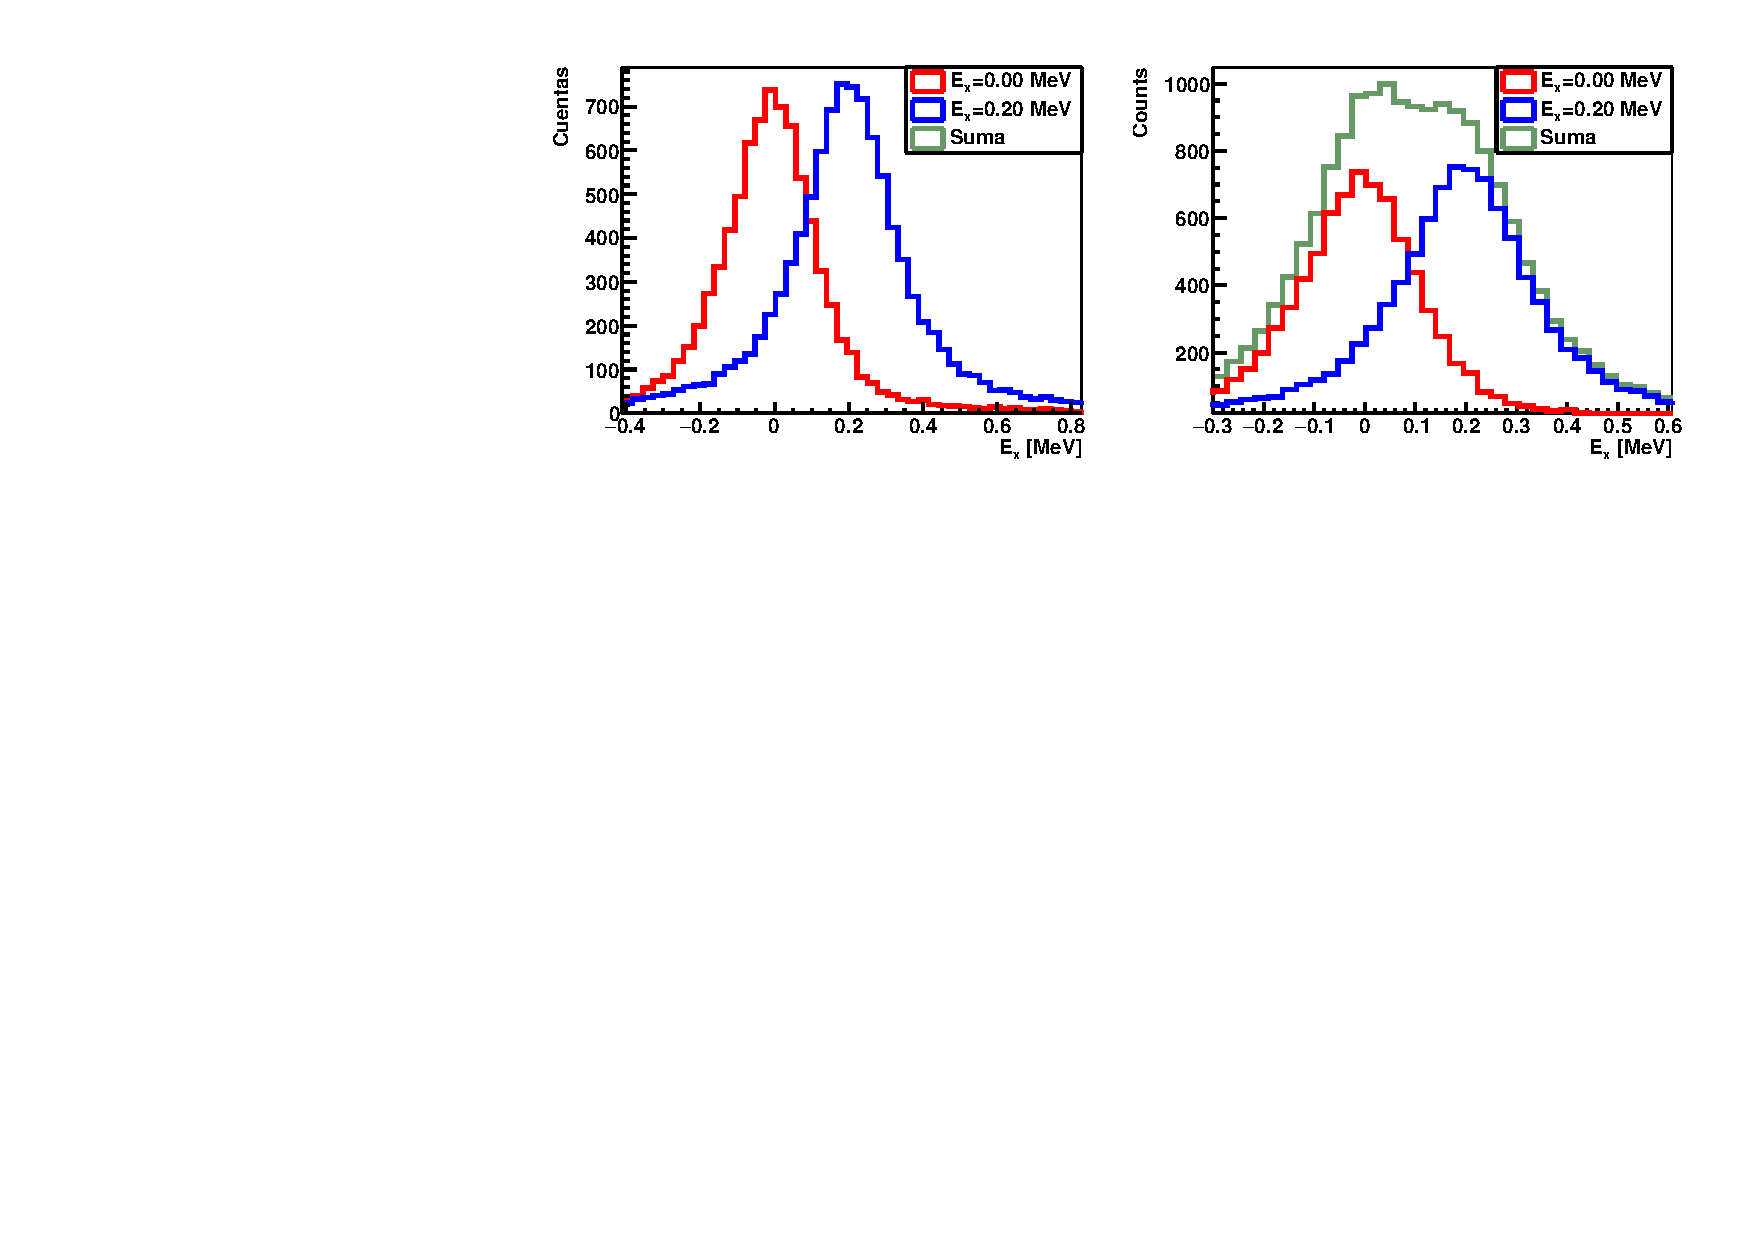
\includegraphics[width=1\textwidth]{Imagenes/Rec_incIdx1_single.pdf}
    \caption{Energía de excitación para $\sigma_{str}$.}
    \label{Fig:05-RecExcIdx1}
\end{figure}

\subsection{Recostrucción solo con stragling angular}

Aquí solo vamos a tener en cuenta el efecto de la dispersión angular, con el cual obtenemos una varianza gaussiana tal que: 

\begin{equation}
    \sigma_{\theta}(0.0) = \num{0.201336762255(0.0006744131)} \ \text{MeV} \quad 
    \sigma_{\theta}(0.2) = \num{0.168440735045(0.0007209796)} \ \text{MeV}
\end{equation} 
con un valor mucho mas grande que el anterior y que como podemos ver en \cref{Tab:05-ExcRec} es prácticamente toda la contribución a $\sigma_{tot}$. En la imagen \cref{Fig:05-RecExcIdx2} podemos ver como ya no diferenciamos los picos en el histograma apilado. Sin embargo, debemos tener en cuenta que el número de 

\vspace*{-0.25cm}
\begin{figure}[H]
    \centering
    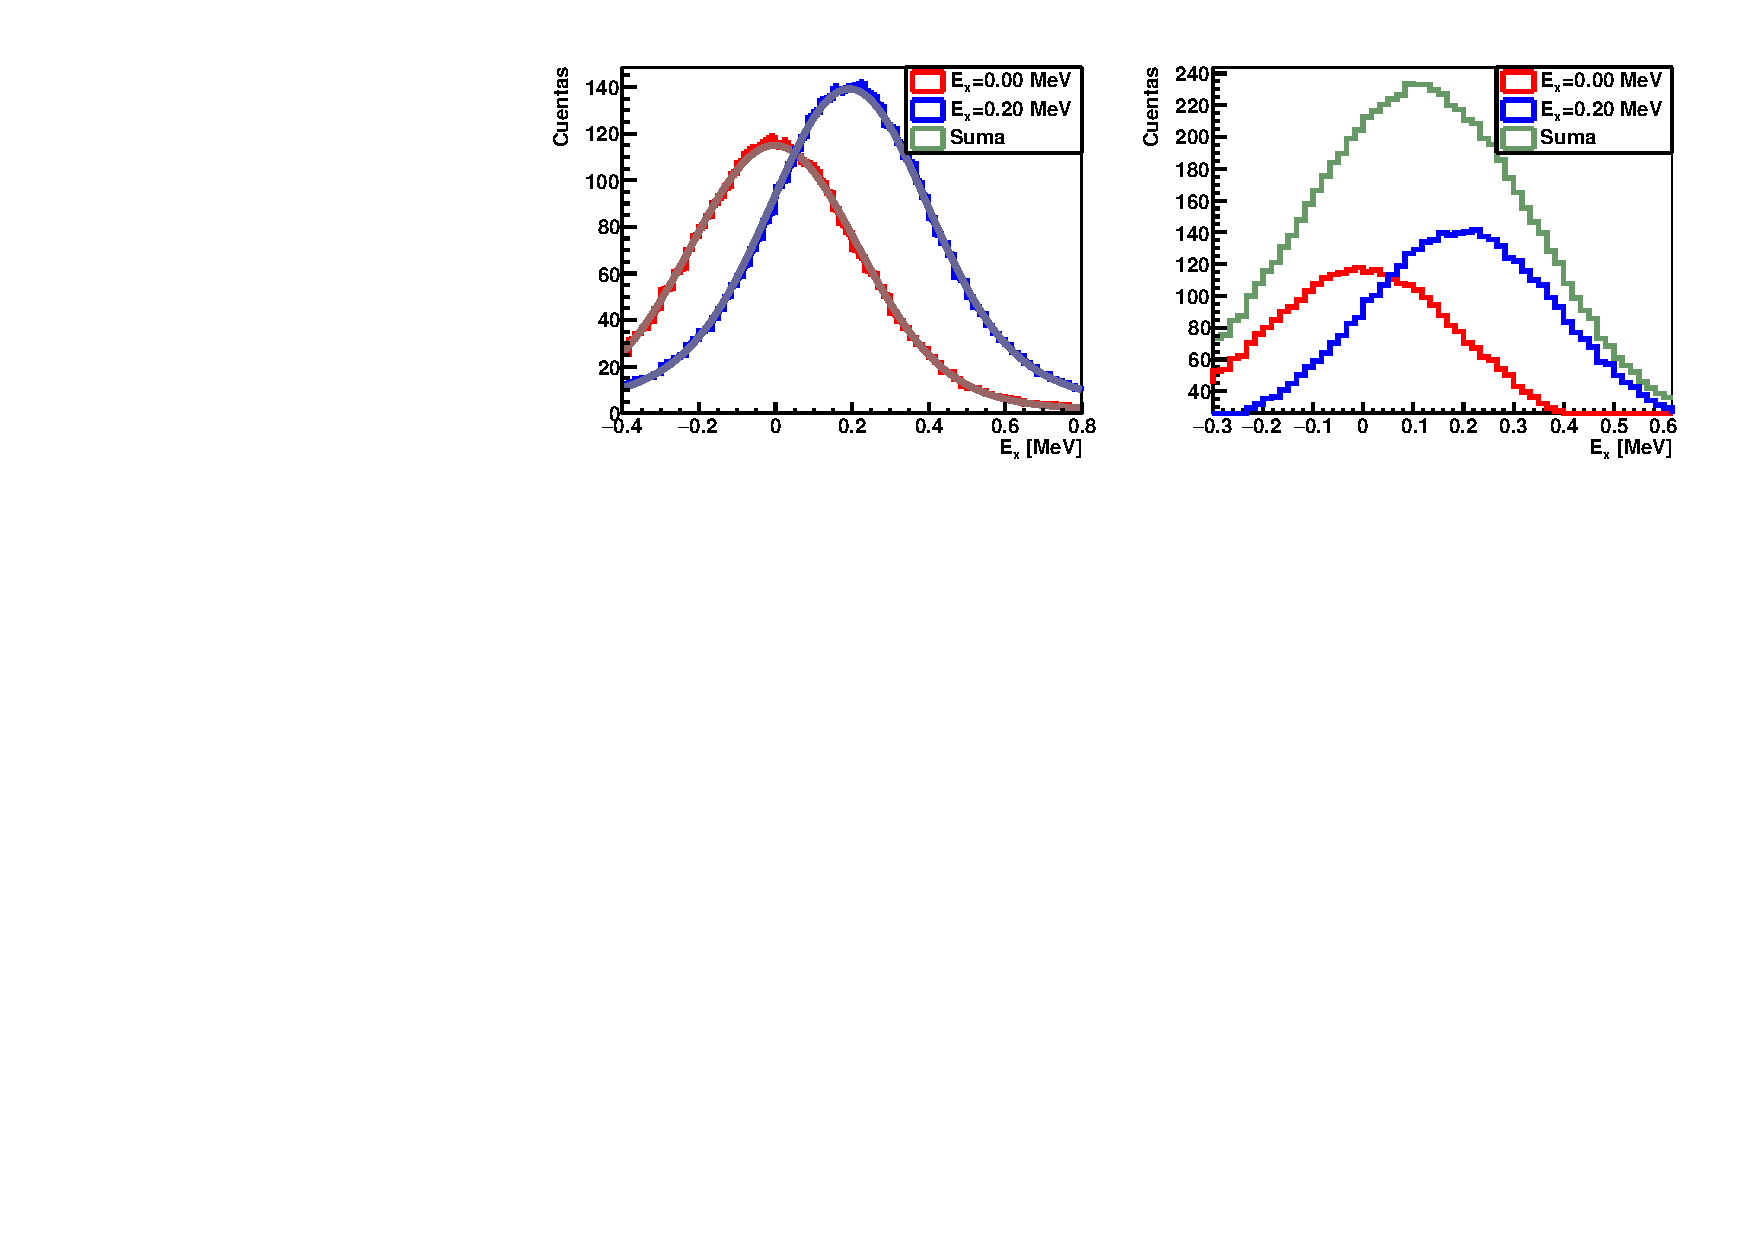
\includegraphics[width=1\textwidth]{Imagenes/Rec_incIdx2_single.pdf}
    \caption{Energía de excitación para $\sigma_{\theta}$.}
    \label{Fig:05-RecExcIdx2}
\end{figure}

\subsection{Recostrucción con todas las fuentes de incertidumbre}

Aquí solo vamos a tener en cuenta todos las fuentes de incertidumbre implementadas, obteniendo así: 

\begin{equation}
    \sigma_{tot}(0.0) =\num{0.219033325961(0.0006865088)} \ \text{MeV} \quad 
    \sigma_{tot}(0.2) = \num{0.179463342520(0.0007321261)} \ \text{MeV}
\end{equation} 
e, igual que en el caso anterior, no podemos distiguir los picos del histograma apilado \cref{Fig:05-RecExcIdx0}. 
\vspace*{-0.25cm}
\begin{figure}[H]
    \centering
    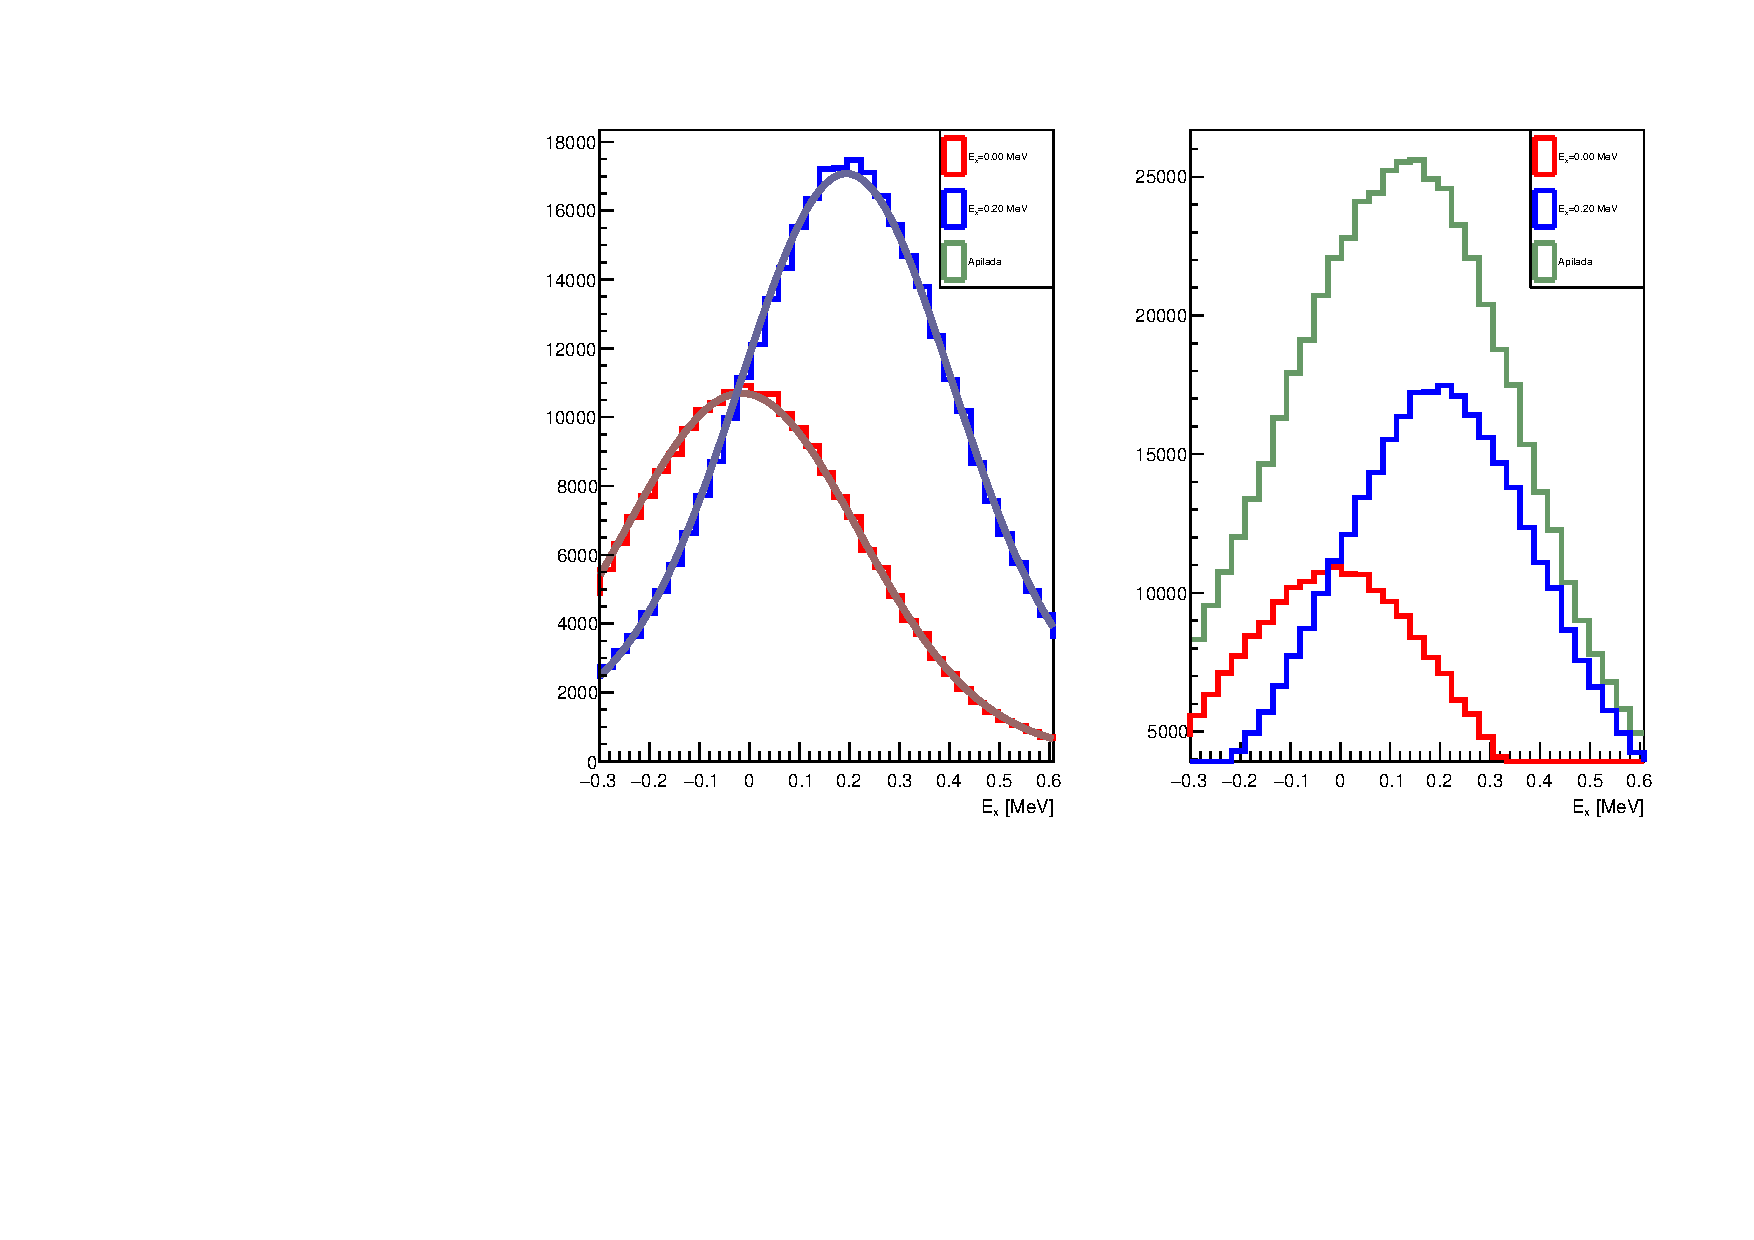
\includegraphics[width=1\textwidth]{Imagenes/Rec_incIdx0_single.pdf}
    \caption{Energía de excitación para $\sigma_{tot}$.}
    \label{Fig:05-RecExcIdx0}
\end{figure}

\subsection{Resumen de resultados}



\begin{table}[H] \centering 
\begin{tabular}{llll} \hline
\toprule 
 & $\sigma(0.0)$ [MeV]  &  $\sigma(0.20)$ [MeV]  \\ \midrule 
$\sigma_{tot}$ & $\num{0.221399220037(0.0021212987)}$ & $\num{0.185196321591(0.0022299371)}$\\ 
$\sigma_{straggling}$ & $\num{0.089228019253(0.0014396243)}$ & $\num{0.066717598649(0.0020985552)}$\\ 
$\sigma_{\theta}$ & $\num{0.202223846486(0.0020712731)}$ & $\num{0.173000700171(0.0022192850)}$\\ 
$\sigma_{0}$ & $\num{0.012904479318(0.0023798058)}$ & $\num{0.018380035441(0.0040286966)}$\\ 
 \bottomrule 
\end{tabular}

\caption{$\sigma$ del ajuste gaussiano a la distribución de energía de excitación recostruida.}
\label{Tab:05-ExcRec}
\end{table}



\newpage
%\appendix
%
\section{Convenciones de Nombres}

En C++, seguir convenciones claras de nombres para las variables, funciones y clases facilita la legibilidad y el mantenimiento del código. A continuación, se presentan las prácticas más comunes en la denominación de distintos elementos.ç
\subsection{Clases}
Las clases suelen seguir la \textbf{Convención PascalCase}, donde cada palabra comienza con mayúscula y no se usan guiones bajos.

\begin{itemize}
\item Ejemplo: \texttt{Particle}, \texttt{CollisionEvent}, \texttt{EnergyCalculator}
\end{itemize}

\subsection{Variables}
\begin{itemize}
\item \textbf{int}: suele usarse \textbf{camelCase}, empezando con minúscula y sin guiones bajos.
\begin{itemize}
\item Ejemplo: \texttt{eventCounter}, \texttt{particleId}
\end{itemize}
\item \textbf{double}: se sigue el mismo esquema \textbf{camelCase}, pero indicando la magnitud si es relevante.
\begin{itemize}
\item Ejemplo: \texttt{beamEnergy}, \texttt{collisionAngle}
\end{itemize}
\item \textbf{bool}: comienza con \texttt{is}, \texttt{has}, \texttt{can}, etc., seguido de PascalCase.
\begin{itemize}
\item Ejemplo: \texttt{isActive}, \texttt{hasCollided}
\end{itemize}
\end{itemize}

\subsection{Constantes}
Las constantes globales o locales usan \textbf{UPPERCASE WITH UNDERSCORES}.

\begin{itemize}
\item Ejemplo: \texttt{PI}, \texttt{MAX PARTICLES}, \texttt{SPEED OF LIGHT}
\end{itemize}

\subsection{Variables que pueden cambiar (mutable)}
Siguen las convenciones generales para \textbf{int} o \textbf{double}, sin notación especial adicional:

\begin{itemize}
\item Ejemplo: \texttt{currentEnergy}, \texttt{numberOfSteps}
\end{itemize}

\subsection{Funciones y Métodos}
Se utiliza \textbf{camelCase}, iniciando en minúscula.

\begin{itemize}
\item Ejemplo: \texttt{calculateEnergy()}, \texttt{setParticleType()}
\end{itemize}

\subsection{Miembros privados de clase}
Se puede usar un guion bajo al final o al principio para diferenciarlos.

\begin{itemize}
\item Ejemplo: \texttt{mass}, \texttt{energy}
\end{itemize}

\subsection{Resumen de estilos}
\begin{tabular}{|c|c|}
\hline
Tipo & Convención de Nombre \\
\hline
Clases & PascalCase \\
Variables (int, double) & camelCase \\
Booleanos & camelCase con prefijos (is, has) \\
Constantes & UPPERCASE WITH UNDERSCORES \\
Funciones & camelCase \\
Miembros privados & camelCase con guion bajo al final o inicio \\
\hline
\end{tabular}
%\newpage 

\printbibliography
\addcontentsline{toc}{section}{Referencias}
			
\end{document}
